\documentclass[11pt]{article}

    \usepackage[breakable]{tcolorbox}
    \usepackage{parskip} % Stop auto-indenting (to mimic markdown behaviour)
    
    \usepackage{iftex}
    \ifPDFTeX
    	\usepackage[T1]{fontenc}
    	\usepackage{mathpazo}
    \else
    	\usepackage{fontspec}
    \fi

    % Basic figure setup, for now with no caption control since it's done
    % automatically by Pandoc (which extracts ![](path) syntax from Markdown).
    \usepackage{graphicx}
    % Maintain compatibility with old templates. Remove in nbconvert 6.0
    \let\Oldincludegraphics\includegraphics
    % Ensure that by default, figures have no caption (until we provide a
    % proper Figure object with a Caption API and a way to capture that
    % in the conversion process - todo).
    \usepackage{caption}
    \DeclareCaptionFormat{nocaption}{}
    \captionsetup{format=nocaption,aboveskip=0pt,belowskip=0pt}

    \usepackage{float}
    \floatplacement{figure}{H} % forces figures to be placed at the correct location
    \usepackage{xcolor} % Allow colors to be defined
    \usepackage{enumerate} % Needed for markdown enumerations to work
    \usepackage{geometry} % Used to adjust the document margins
    \usepackage{amsmath} % Equations
    \usepackage{amssymb} % Equations
    \usepackage{textcomp} % defines textquotesingle
    % Hack from http://tex.stackexchange.com/a/47451/13684:
    \AtBeginDocument{%
        \def\PYZsq{\textquotesingle}% Upright quotes in Pygmentized code
    }
    \usepackage{upquote} % Upright quotes for verbatim code
    \usepackage{eurosym} % defines \euro
    \usepackage[mathletters]{ucs} % Extended unicode (utf-8) support
    \usepackage{fancyvrb} % verbatim replacement that allows latex
    \usepackage{grffile} % extends the file name processing of package graphics 
                         % to support a larger range
    \makeatletter % fix for old versions of grffile with XeLaTeX
    \@ifpackagelater{grffile}{2019/11/01}
    {
      % Do nothing on new versions
    }
    {
      \def\Gread@@xetex#1{%
        \IfFileExists{"\Gin@base".bb}%
        {\Gread@eps{\Gin@base.bb}}%
        {\Gread@@xetex@aux#1}%
      }
    }
    \makeatother
    \usepackage[Export]{adjustbox} % Used to constrain images to a maximum size
    \adjustboxset{max size={0.9\linewidth}{0.9\paperheight}}

    % The hyperref package gives us a pdf with properly built
    % internal navigation ('pdf bookmarks' for the table of contents,
    % internal cross-reference links, web links for URLs, etc.)
    \usepackage{hyperref}
    % The default LaTeX title has an obnoxious amount of whitespace. By default,
    % titling removes some of it. It also provides customization options.
    \usepackage{titling}
    \usepackage{longtable} % longtable support required by pandoc >1.10
    \usepackage{booktabs}  % table support for pandoc > 1.12.2
    \usepackage[inline]{enumitem} % IRkernel/repr support (it uses the enumerate* environment)
    \usepackage[normalem]{ulem} % ulem is needed to support strikethroughs (\sout)
                                % normalem makes italics be italics, not underlines
    \usepackage{mathrsfs}
    

    
    % Colors for the hyperref package
    \definecolor{urlcolor}{rgb}{0,.145,.698}
    \definecolor{linkcolor}{rgb}{.71,0.21,0.01}
    \definecolor{citecolor}{rgb}{.12,.54,.11}

    % ANSI colors
    \definecolor{ansi-black}{HTML}{3E424D}
    \definecolor{ansi-black-intense}{HTML}{282C36}
    \definecolor{ansi-red}{HTML}{E75C58}
    \definecolor{ansi-red-intense}{HTML}{B22B31}
    \definecolor{ansi-green}{HTML}{00A250}
    \definecolor{ansi-green-intense}{HTML}{007427}
    \definecolor{ansi-yellow}{HTML}{DDB62B}
    \definecolor{ansi-yellow-intense}{HTML}{B27D12}
    \definecolor{ansi-blue}{HTML}{208FFB}
    \definecolor{ansi-blue-intense}{HTML}{0065CA}
    \definecolor{ansi-magenta}{HTML}{D160C4}
    \definecolor{ansi-magenta-intense}{HTML}{A03196}
    \definecolor{ansi-cyan}{HTML}{60C6C8}
    \definecolor{ansi-cyan-intense}{HTML}{258F8F}
    \definecolor{ansi-white}{HTML}{C5C1B4}
    \definecolor{ansi-white-intense}{HTML}{A1A6B2}
    \definecolor{ansi-default-inverse-fg}{HTML}{FFFFFF}
    \definecolor{ansi-default-inverse-bg}{HTML}{000000}

    % common color for the border for error outputs.
    \definecolor{outerrorbackground}{HTML}{FFDFDF}

    % commands and environments needed by pandoc snippets
    % extracted from the output of `pandoc -s`
    \providecommand{\tightlist}{%
      \setlength{\itemsep}{0pt}\setlength{\parskip}{0pt}}
    \DefineVerbatimEnvironment{Highlighting}{Verbatim}{commandchars=\\\{\}}
    % Add ',fontsize=\small' for more characters per line
    \newenvironment{Shaded}{}{}
    \newcommand{\KeywordTok}[1]{\textcolor[rgb]{0.00,0.44,0.13}{\textbf{{#1}}}}
    \newcommand{\DataTypeTok}[1]{\textcolor[rgb]{0.56,0.13,0.00}{{#1}}}
    \newcommand{\DecValTok}[1]{\textcolor[rgb]{0.25,0.63,0.44}{{#1}}}
    \newcommand{\BaseNTok}[1]{\textcolor[rgb]{0.25,0.63,0.44}{{#1}}}
    \newcommand{\FloatTok}[1]{\textcolor[rgb]{0.25,0.63,0.44}{{#1}}}
    \newcommand{\CharTok}[1]{\textcolor[rgb]{0.25,0.44,0.63}{{#1}}}
    \newcommand{\StringTok}[1]{\textcolor[rgb]{0.25,0.44,0.63}{{#1}}}
    \newcommand{\CommentTok}[1]{\textcolor[rgb]{0.38,0.63,0.69}{\textit{{#1}}}}
    \newcommand{\OtherTok}[1]{\textcolor[rgb]{0.00,0.44,0.13}{{#1}}}
    \newcommand{\AlertTok}[1]{\textcolor[rgb]{1.00,0.00,0.00}{\textbf{{#1}}}}
    \newcommand{\FunctionTok}[1]{\textcolor[rgb]{0.02,0.16,0.49}{{#1}}}
    \newcommand{\RegionMarkerTok}[1]{{#1}}
    \newcommand{\ErrorTok}[1]{\textcolor[rgb]{1.00,0.00,0.00}{\textbf{{#1}}}}
    \newcommand{\NormalTok}[1]{{#1}}
    
    % Additional commands for more recent versions of Pandoc
    \newcommand{\ConstantTok}[1]{\textcolor[rgb]{0.53,0.00,0.00}{{#1}}}
    \newcommand{\SpecialCharTok}[1]{\textcolor[rgb]{0.25,0.44,0.63}{{#1}}}
    \newcommand{\VerbatimStringTok}[1]{\textcolor[rgb]{0.25,0.44,0.63}{{#1}}}
    \newcommand{\SpecialStringTok}[1]{\textcolor[rgb]{0.73,0.40,0.53}{{#1}}}
    \newcommand{\ImportTok}[1]{{#1}}
    \newcommand{\DocumentationTok}[1]{\textcolor[rgb]{0.73,0.13,0.13}{\textit{{#1}}}}
    \newcommand{\AnnotationTok}[1]{\textcolor[rgb]{0.38,0.63,0.69}{\textbf{\textit{{#1}}}}}
    \newcommand{\CommentVarTok}[1]{\textcolor[rgb]{0.38,0.63,0.69}{\textbf{\textit{{#1}}}}}
    \newcommand{\VariableTok}[1]{\textcolor[rgb]{0.10,0.09,0.49}{{#1}}}
    \newcommand{\ControlFlowTok}[1]{\textcolor[rgb]{0.00,0.44,0.13}{\textbf{{#1}}}}
    \newcommand{\OperatorTok}[1]{\textcolor[rgb]{0.40,0.40,0.40}{{#1}}}
    \newcommand{\BuiltInTok}[1]{{#1}}
    \newcommand{\ExtensionTok}[1]{{#1}}
    \newcommand{\PreprocessorTok}[1]{\textcolor[rgb]{0.74,0.48,0.00}{{#1}}}
    \newcommand{\AttributeTok}[1]{\textcolor[rgb]{0.49,0.56,0.16}{{#1}}}
    \newcommand{\InformationTok}[1]{\textcolor[rgb]{0.38,0.63,0.69}{\textbf{\textit{{#1}}}}}
    \newcommand{\WarningTok}[1]{\textcolor[rgb]{0.38,0.63,0.69}{\textbf{\textit{{#1}}}}}
    
    
    % Define a nice break command that doesn't care if a line doesn't already
    % exist.
    \def\br{\hspace*{\fill} \\* }
    % Math Jax compatibility definitions
    \def\gt{>}
    \def\lt{<}
    \let\Oldtex\TeX
    \let\Oldlatex\LaTeX
    \renewcommand{\TeX}{\textrm{\Oldtex}}
    \renewcommand{\LaTeX}{\textrm{\Oldlatex}}
    % Document parameters
    % Document title
    \title{introduction-to-text-analysis-with-python}
    
    
    
    
    
% Pygments definitions
\makeatletter
\def\PY@reset{\let\PY@it=\relax \let\PY@bf=\relax%
    \let\PY@ul=\relax \let\PY@tc=\relax%
    \let\PY@bc=\relax \let\PY@ff=\relax}
\def\PY@tok#1{\csname PY@tok@#1\endcsname}
\def\PY@toks#1+{\ifx\relax#1\empty\else%
    \PY@tok{#1}\expandafter\PY@toks\fi}
\def\PY@do#1{\PY@bc{\PY@tc{\PY@ul{%
    \PY@it{\PY@bf{\PY@ff{#1}}}}}}}
\def\PY#1#2{\PY@reset\PY@toks#1+\relax+\PY@do{#2}}

\@namedef{PY@tok@w}{\def\PY@tc##1{\textcolor[rgb]{0.73,0.73,0.73}{##1}}}
\@namedef{PY@tok@c}{\let\PY@it=\textit\def\PY@tc##1{\textcolor[rgb]{0.25,0.50,0.50}{##1}}}
\@namedef{PY@tok@cp}{\def\PY@tc##1{\textcolor[rgb]{0.74,0.48,0.00}{##1}}}
\@namedef{PY@tok@k}{\let\PY@bf=\textbf\def\PY@tc##1{\textcolor[rgb]{0.00,0.50,0.00}{##1}}}
\@namedef{PY@tok@kp}{\def\PY@tc##1{\textcolor[rgb]{0.00,0.50,0.00}{##1}}}
\@namedef{PY@tok@kt}{\def\PY@tc##1{\textcolor[rgb]{0.69,0.00,0.25}{##1}}}
\@namedef{PY@tok@o}{\def\PY@tc##1{\textcolor[rgb]{0.40,0.40,0.40}{##1}}}
\@namedef{PY@tok@ow}{\let\PY@bf=\textbf\def\PY@tc##1{\textcolor[rgb]{0.67,0.13,1.00}{##1}}}
\@namedef{PY@tok@nb}{\def\PY@tc##1{\textcolor[rgb]{0.00,0.50,0.00}{##1}}}
\@namedef{PY@tok@nf}{\def\PY@tc##1{\textcolor[rgb]{0.00,0.00,1.00}{##1}}}
\@namedef{PY@tok@nc}{\let\PY@bf=\textbf\def\PY@tc##1{\textcolor[rgb]{0.00,0.00,1.00}{##1}}}
\@namedef{PY@tok@nn}{\let\PY@bf=\textbf\def\PY@tc##1{\textcolor[rgb]{0.00,0.00,1.00}{##1}}}
\@namedef{PY@tok@ne}{\let\PY@bf=\textbf\def\PY@tc##1{\textcolor[rgb]{0.82,0.25,0.23}{##1}}}
\@namedef{PY@tok@nv}{\def\PY@tc##1{\textcolor[rgb]{0.10,0.09,0.49}{##1}}}
\@namedef{PY@tok@no}{\def\PY@tc##1{\textcolor[rgb]{0.53,0.00,0.00}{##1}}}
\@namedef{PY@tok@nl}{\def\PY@tc##1{\textcolor[rgb]{0.63,0.63,0.00}{##1}}}
\@namedef{PY@tok@ni}{\let\PY@bf=\textbf\def\PY@tc##1{\textcolor[rgb]{0.60,0.60,0.60}{##1}}}
\@namedef{PY@tok@na}{\def\PY@tc##1{\textcolor[rgb]{0.49,0.56,0.16}{##1}}}
\@namedef{PY@tok@nt}{\let\PY@bf=\textbf\def\PY@tc##1{\textcolor[rgb]{0.00,0.50,0.00}{##1}}}
\@namedef{PY@tok@nd}{\def\PY@tc##1{\textcolor[rgb]{0.67,0.13,1.00}{##1}}}
\@namedef{PY@tok@s}{\def\PY@tc##1{\textcolor[rgb]{0.73,0.13,0.13}{##1}}}
\@namedef{PY@tok@sd}{\let\PY@it=\textit\def\PY@tc##1{\textcolor[rgb]{0.73,0.13,0.13}{##1}}}
\@namedef{PY@tok@si}{\let\PY@bf=\textbf\def\PY@tc##1{\textcolor[rgb]{0.73,0.40,0.53}{##1}}}
\@namedef{PY@tok@se}{\let\PY@bf=\textbf\def\PY@tc##1{\textcolor[rgb]{0.73,0.40,0.13}{##1}}}
\@namedef{PY@tok@sr}{\def\PY@tc##1{\textcolor[rgb]{0.73,0.40,0.53}{##1}}}
\@namedef{PY@tok@ss}{\def\PY@tc##1{\textcolor[rgb]{0.10,0.09,0.49}{##1}}}
\@namedef{PY@tok@sx}{\def\PY@tc##1{\textcolor[rgb]{0.00,0.50,0.00}{##1}}}
\@namedef{PY@tok@m}{\def\PY@tc##1{\textcolor[rgb]{0.40,0.40,0.40}{##1}}}
\@namedef{PY@tok@gh}{\let\PY@bf=\textbf\def\PY@tc##1{\textcolor[rgb]{0.00,0.00,0.50}{##1}}}
\@namedef{PY@tok@gu}{\let\PY@bf=\textbf\def\PY@tc##1{\textcolor[rgb]{0.50,0.00,0.50}{##1}}}
\@namedef{PY@tok@gd}{\def\PY@tc##1{\textcolor[rgb]{0.63,0.00,0.00}{##1}}}
\@namedef{PY@tok@gi}{\def\PY@tc##1{\textcolor[rgb]{0.00,0.63,0.00}{##1}}}
\@namedef{PY@tok@gr}{\def\PY@tc##1{\textcolor[rgb]{1.00,0.00,0.00}{##1}}}
\@namedef{PY@tok@ge}{\let\PY@it=\textit}
\@namedef{PY@tok@gs}{\let\PY@bf=\textbf}
\@namedef{PY@tok@gp}{\let\PY@bf=\textbf\def\PY@tc##1{\textcolor[rgb]{0.00,0.00,0.50}{##1}}}
\@namedef{PY@tok@go}{\def\PY@tc##1{\textcolor[rgb]{0.53,0.53,0.53}{##1}}}
\@namedef{PY@tok@gt}{\def\PY@tc##1{\textcolor[rgb]{0.00,0.27,0.87}{##1}}}
\@namedef{PY@tok@err}{\def\PY@bc##1{{\setlength{\fboxsep}{\string -\fboxrule}\fcolorbox[rgb]{1.00,0.00,0.00}{1,1,1}{\strut ##1}}}}
\@namedef{PY@tok@kc}{\let\PY@bf=\textbf\def\PY@tc##1{\textcolor[rgb]{0.00,0.50,0.00}{##1}}}
\@namedef{PY@tok@kd}{\let\PY@bf=\textbf\def\PY@tc##1{\textcolor[rgb]{0.00,0.50,0.00}{##1}}}
\@namedef{PY@tok@kn}{\let\PY@bf=\textbf\def\PY@tc##1{\textcolor[rgb]{0.00,0.50,0.00}{##1}}}
\@namedef{PY@tok@kr}{\let\PY@bf=\textbf\def\PY@tc##1{\textcolor[rgb]{0.00,0.50,0.00}{##1}}}
\@namedef{PY@tok@bp}{\def\PY@tc##1{\textcolor[rgb]{0.00,0.50,0.00}{##1}}}
\@namedef{PY@tok@fm}{\def\PY@tc##1{\textcolor[rgb]{0.00,0.00,1.00}{##1}}}
\@namedef{PY@tok@vc}{\def\PY@tc##1{\textcolor[rgb]{0.10,0.09,0.49}{##1}}}
\@namedef{PY@tok@vg}{\def\PY@tc##1{\textcolor[rgb]{0.10,0.09,0.49}{##1}}}
\@namedef{PY@tok@vi}{\def\PY@tc##1{\textcolor[rgb]{0.10,0.09,0.49}{##1}}}
\@namedef{PY@tok@vm}{\def\PY@tc##1{\textcolor[rgb]{0.10,0.09,0.49}{##1}}}
\@namedef{PY@tok@sa}{\def\PY@tc##1{\textcolor[rgb]{0.73,0.13,0.13}{##1}}}
\@namedef{PY@tok@sb}{\def\PY@tc##1{\textcolor[rgb]{0.73,0.13,0.13}{##1}}}
\@namedef{PY@tok@sc}{\def\PY@tc##1{\textcolor[rgb]{0.73,0.13,0.13}{##1}}}
\@namedef{PY@tok@dl}{\def\PY@tc##1{\textcolor[rgb]{0.73,0.13,0.13}{##1}}}
\@namedef{PY@tok@s2}{\def\PY@tc##1{\textcolor[rgb]{0.73,0.13,0.13}{##1}}}
\@namedef{PY@tok@sh}{\def\PY@tc##1{\textcolor[rgb]{0.73,0.13,0.13}{##1}}}
\@namedef{PY@tok@s1}{\def\PY@tc##1{\textcolor[rgb]{0.73,0.13,0.13}{##1}}}
\@namedef{PY@tok@mb}{\def\PY@tc##1{\textcolor[rgb]{0.40,0.40,0.40}{##1}}}
\@namedef{PY@tok@mf}{\def\PY@tc##1{\textcolor[rgb]{0.40,0.40,0.40}{##1}}}
\@namedef{PY@tok@mh}{\def\PY@tc##1{\textcolor[rgb]{0.40,0.40,0.40}{##1}}}
\@namedef{PY@tok@mi}{\def\PY@tc##1{\textcolor[rgb]{0.40,0.40,0.40}{##1}}}
\@namedef{PY@tok@il}{\def\PY@tc##1{\textcolor[rgb]{0.40,0.40,0.40}{##1}}}
\@namedef{PY@tok@mo}{\def\PY@tc##1{\textcolor[rgb]{0.40,0.40,0.40}{##1}}}
\@namedef{PY@tok@ch}{\let\PY@it=\textit\def\PY@tc##1{\textcolor[rgb]{0.25,0.50,0.50}{##1}}}
\@namedef{PY@tok@cm}{\let\PY@it=\textit\def\PY@tc##1{\textcolor[rgb]{0.25,0.50,0.50}{##1}}}
\@namedef{PY@tok@cpf}{\let\PY@it=\textit\def\PY@tc##1{\textcolor[rgb]{0.25,0.50,0.50}{##1}}}
\@namedef{PY@tok@c1}{\let\PY@it=\textit\def\PY@tc##1{\textcolor[rgb]{0.25,0.50,0.50}{##1}}}
\@namedef{PY@tok@cs}{\let\PY@it=\textit\def\PY@tc##1{\textcolor[rgb]{0.25,0.50,0.50}{##1}}}

\def\PYZbs{\char`\\}
\def\PYZus{\char`\_}
\def\PYZob{\char`\{}
\def\PYZcb{\char`\}}
\def\PYZca{\char`\^}
\def\PYZam{\char`\&}
\def\PYZlt{\char`\<}
\def\PYZgt{\char`\>}
\def\PYZsh{\char`\#}
\def\PYZpc{\char`\%}
\def\PYZdl{\char`\$}
\def\PYZhy{\char`\-}
\def\PYZsq{\char`\'}
\def\PYZdq{\char`\"}
\def\PYZti{\char`\~}
% for compatibility with earlier versions
\def\PYZat{@}
\def\PYZlb{[}
\def\PYZrb{]}
\makeatother


    % For linebreaks inside Verbatim environment from package fancyvrb. 
    \makeatletter
        \newbox\Wrappedcontinuationbox 
        \newbox\Wrappedvisiblespacebox 
        \newcommand*\Wrappedvisiblespace {\textcolor{red}{\textvisiblespace}} 
        \newcommand*\Wrappedcontinuationsymbol {\textcolor{red}{\llap{\tiny$\m@th\hookrightarrow$}}} 
        \newcommand*\Wrappedcontinuationindent {3ex } 
        \newcommand*\Wrappedafterbreak {\kern\Wrappedcontinuationindent\copy\Wrappedcontinuationbox} 
        % Take advantage of the already applied Pygments mark-up to insert 
        % potential linebreaks for TeX processing. 
        %        {, <, #, %, $, ' and ": go to next line. 
        %        _, }, ^, &, >, - and ~: stay at end of broken line. 
        % Use of \textquotesingle for straight quote. 
        \newcommand*\Wrappedbreaksatspecials {% 
            \def\PYGZus{\discretionary{\char`\_}{\Wrappedafterbreak}{\char`\_}}% 
            \def\PYGZob{\discretionary{}{\Wrappedafterbreak\char`\{}{\char`\{}}% 
            \def\PYGZcb{\discretionary{\char`\}}{\Wrappedafterbreak}{\char`\}}}% 
            \def\PYGZca{\discretionary{\char`\^}{\Wrappedafterbreak}{\char`\^}}% 
            \def\PYGZam{\discretionary{\char`\&}{\Wrappedafterbreak}{\char`\&}}% 
            \def\PYGZlt{\discretionary{}{\Wrappedafterbreak\char`\<}{\char`\<}}% 
            \def\PYGZgt{\discretionary{\char`\>}{\Wrappedafterbreak}{\char`\>}}% 
            \def\PYGZsh{\discretionary{}{\Wrappedafterbreak\char`\#}{\char`\#}}% 
            \def\PYGZpc{\discretionary{}{\Wrappedafterbreak\char`\%}{\char`\%}}% 
            \def\PYGZdl{\discretionary{}{\Wrappedafterbreak\char`\$}{\char`\$}}% 
            \def\PYGZhy{\discretionary{\char`\-}{\Wrappedafterbreak}{\char`\-}}% 
            \def\PYGZsq{\discretionary{}{\Wrappedafterbreak\textquotesingle}{\textquotesingle}}% 
            \def\PYGZdq{\discretionary{}{\Wrappedafterbreak\char`\"}{\char`\"}}% 
            \def\PYGZti{\discretionary{\char`\~}{\Wrappedafterbreak}{\char`\~}}% 
        } 
        % Some characters . , ; ? ! / are not pygmentized. 
        % This macro makes them "active" and they will insert potential linebreaks 
        \newcommand*\Wrappedbreaksatpunct {% 
            \lccode`\~`\.\lowercase{\def~}{\discretionary{\hbox{\char`\.}}{\Wrappedafterbreak}{\hbox{\char`\.}}}% 
            \lccode`\~`\,\lowercase{\def~}{\discretionary{\hbox{\char`\,}}{\Wrappedafterbreak}{\hbox{\char`\,}}}% 
            \lccode`\~`\;\lowercase{\def~}{\discretionary{\hbox{\char`\;}}{\Wrappedafterbreak}{\hbox{\char`\;}}}% 
            \lccode`\~`\:\lowercase{\def~}{\discretionary{\hbox{\char`\:}}{\Wrappedafterbreak}{\hbox{\char`\:}}}% 
            \lccode`\~`\?\lowercase{\def~}{\discretionary{\hbox{\char`\?}}{\Wrappedafterbreak}{\hbox{\char`\?}}}% 
            \lccode`\~`\!\lowercase{\def~}{\discretionary{\hbox{\char`\!}}{\Wrappedafterbreak}{\hbox{\char`\!}}}% 
            \lccode`\~`\/\lowercase{\def~}{\discretionary{\hbox{\char`\/}}{\Wrappedafterbreak}{\hbox{\char`\/}}}% 
            \catcode`\.\active
            \catcode`\,\active 
            \catcode`\;\active
            \catcode`\:\active
            \catcode`\?\active
            \catcode`\!\active
            \catcode`\/\active 
            \lccode`\~`\~ 	
        }
    \makeatother

    \let\OriginalVerbatim=\Verbatim
    \makeatletter
    \renewcommand{\Verbatim}[1][1]{%
        %\parskip\z@skip
        \sbox\Wrappedcontinuationbox {\Wrappedcontinuationsymbol}%
        \sbox\Wrappedvisiblespacebox {\FV@SetupFont\Wrappedvisiblespace}%
        \def\FancyVerbFormatLine ##1{\hsize\linewidth
            \vtop{\raggedright\hyphenpenalty\z@\exhyphenpenalty\z@
                \doublehyphendemerits\z@\finalhyphendemerits\z@
                \strut ##1\strut}%
        }%
        % If the linebreak is at a space, the latter will be displayed as visible
        % space at end of first line, and a continuation symbol starts next line.
        % Stretch/shrink are however usually zero for typewriter font.
        \def\FV@Space {%
            \nobreak\hskip\z@ plus\fontdimen3\font minus\fontdimen4\font
            \discretionary{\copy\Wrappedvisiblespacebox}{\Wrappedafterbreak}
            {\kern\fontdimen2\font}%
        }%
        
        % Allow breaks at special characters using \PYG... macros.
        \Wrappedbreaksatspecials
        % Breaks at punctuation characters . , ; ? ! and / need catcode=\active 	
        \OriginalVerbatim[#1,codes*=\Wrappedbreaksatpunct]%
    }
    \makeatother

    % Exact colors from NB
    \definecolor{incolor}{HTML}{303F9F}
    \definecolor{outcolor}{HTML}{D84315}
    \definecolor{cellborder}{HTML}{CFCFCF}
    \definecolor{cellbackground}{HTML}{F7F7F7}
    
    % prompt
    \makeatletter
    \newcommand{\boxspacing}{\kern\kvtcb@left@rule\kern\kvtcb@boxsep}
    \makeatother
    \newcommand{\prompt}[4]{
        {\ttfamily\llap{{\color{#2}[#3]:\hspace{3pt}#4}}\vspace{-\baselineskip}}
    }
    

    
    % Prevent overflowing lines due to hard-to-break entities
    \sloppy 
    % Setup hyperref package
    \hypersetup{
      breaklinks=true,  % so long urls are correctly broken across lines
      colorlinks=true,
      urlcolor=urlcolor,
      linkcolor=linkcolor,
      citecolor=citecolor,
      }
    % Slightly bigger margins than the latex defaults
    
    \geometry{verbose,tmargin=1in,bmargin=1in,lmargin=1in,rmargin=1in}
    
    

\begin{document}
    
    \maketitle
    
    

    
    Run in Google Colab

    \hypertarget{basic-text-analysis-with-python}{%
\section{Basic Text Analysis with
Python}\label{basic-text-analysis-with-python}}

    \hypertarget{introduction}{%
\subsection{Introduction}\label{introduction}}

Text is one of the most widespread forms of sequence data. It can be
understood as either a sequence of characters or a sequence of words,
but it's most common to work at the level of words. According to
industry estimates, only 21\% of the available data is present in a
structured form. Data is being generated as we speak, as we tweet, as we
send messages on WhatsApp and in various other activities. The majority
of this data exists in the textual form, which is highly unstructured in
nature.

Despite having high dimension data, the information present in it is not
directly accessible unless it is processed (read and understood)
manually or analyzed by an automated system. In order to produce
significant and actionable insights from text data, it is important to
get acquainted with the basics of Text Analysis.

    \hypertarget{package-required}{%
\subsection{Package Required}\label{package-required}}

    \textbf{To start}, install the packages you need to run the code in this
notebook.

    \begin{tcolorbox}[breakable, size=fbox, boxrule=1pt, pad at break*=1mm,colback=cellbackground, colframe=cellborder]
\prompt{In}{incolor}{ }{\boxspacing}
\begin{Verbatim}[commandchars=\\\{\}]
\PY{c+c1}{\PYZsh{} Python Regular Expression (RegEx)}
\PY{k+kn}{import} \PY{n+nn}{re}
\PY{c+c1}{\PYZsh{} Operating System Module}
\PY{k+kn}{import} \PY{n+nn}{os}
\PY{c+c1}{\PYZsh{} numpy library}
\PY{k+kn}{import} \PY{n+nn}{numpy} \PY{k}{as} \PY{n+nn}{np}
\PY{c+c1}{\PYZsh{} pandas library}
\PY{k+kn}{import} \PY{n+nn}{pandas} \PY{k}{as} \PY{n+nn}{pd}
\PY{c+c1}{\PYZsh{} matplotlib library}
\PY{k+kn}{import} \PY{n+nn}{matplotlib}\PY{n+nn}{.}\PY{n+nn}{pyplot} \PY{k}{as} \PY{n+nn}{plt}
\PY{c+c1}{\PYZsh{} if uising a Jupyter notebook, include:}
\PY{o}{\PYZpc{}}\PY{k}{matplotlib} inline
\PY{c+c1}{\PYZsh{} Natural Language Toolkit }
\PY{k+kn}{import} \PY{n+nn}{nltk}
\PY{c+c1}{\PYZsh{} The BeautifulSoup Library for WEB Scraping}
\PY{k+kn}{from} \PY{n+nn}{bs4} \PY{k+kn}{import} \PY{n}{BeautifulSoup}

\PY{k+kn}{import} \PY{n+nn}{codecs}
\PY{k+kn}{from} \PY{n+nn}{sklearn} \PY{k+kn}{import} \PY{n}{feature\PYZus{}extraction}
\end{Verbatim}
\end{tcolorbox}

    \hypertarget{definitions}{%
\subsection{Definitions}\label{definitions}}

    \hypertarget{corpus}{%
\subsubsection{Corpus}\label{corpus}}

A Corpus is defined as a \textbf{collection of text documents} for
example a data set containing news is a corpus or the tweets containing
Twitter data is a corpus. So corpus consists of documents, documents
comprise paragraphs, paragraphs comprise sentences and sentences
comprise further smaller units which are called Tokens.

    \hypertarget{using-nltk-corpus}{%
\subsubsection{Using NLTK Corpus}\label{using-nltk-corpus}}

    \hypertarget{loading-your-own-corpus}{%
\subsubsection{Loading Your Own Corpus}\label{loading-your-own-corpus}}

If you have your own collection of text files that you would like to
access using the above methods, you can easily load them with the help
of NLTK's \texttt{PlaintextCorpusReader}. Check the location of your
files on your file system; in the following example, we have taken this
to be the directory
\texttt{C:\textbackslash{}Corpus\textbackslash{}EBA}. Whatever the
location, set this to be the value of corpus\_root.

The second parameter of the PlaintextCorpusReader initializer can be a
list of fileids, like {[}`a.txt', `test/b.txt'{]}, or a pattern that
matches all fileids, like '{[}abc{]}/.*.txt'

    \begin{tcolorbox}[breakable, size=fbox, boxrule=1pt, pad at break*=1mm,colback=cellbackground, colframe=cellborder]
\prompt{In}{incolor}{ }{\boxspacing}
\begin{Verbatim}[commandchars=\\\{\}]
\PY{k+kn}{import} \PY{n+nn}{nltk}
\PY{k+kn}{from} \PY{n+nn}{nltk}\PY{n+nn}{.}\PY{n+nn}{corpus} \PY{k+kn}{import} \PY{n}{PlaintextCorpusReader}

\PY{n}{corpus\PYZus{}root} \PY{o}{=} \PY{l+s+s1}{\PYZsq{}}\PY{l+s+s1}{.}\PY{l+s+s1}{\PYZbs{}}\PY{l+s+s1}{corpus}\PY{l+s+s1}{\PYZbs{}}\PY{l+s+s1}{EBA}\PY{l+s+s1}{\PYZsq{}}
\PY{n}{corpus\PYZus{}list} \PY{o}{=} \PY{n}{PlaintextCorpusReader}\PY{p}{(}\PY{n}{corpus\PYZus{}root}\PY{p}{,} \PY{l+s+s1}{\PYZsq{}}\PY{l+s+s1}{.*}\PY{l+s+s1}{\PYZsq{}}\PY{p}{,} \PY{n}{encoding}\PY{o}{=}\PY{l+s+s1}{\PYZsq{}}\PY{l+s+s1}{latin\PYZhy{}1}\PY{l+s+s1}{\PYZsq{}}\PY{p}{)}
\PY{n}{corpus\PYZus{}list}\PY{o}{.}\PY{n}{fileids}\PY{p}{(}\PY{p}{)}
\end{Verbatim}
\end{tcolorbox}

    Let's pick out one of these text (for example the guideline on the
interest rate), give it a short name, irrbb\ldots{}

    \begin{tcolorbox}[breakable, size=fbox, boxrule=1pt, pad at break*=1mm,colback=cellbackground, colframe=cellborder]
\prompt{In}{incolor}{ }{\boxspacing}
\begin{Verbatim}[commandchars=\\\{\}]
\PY{n+nb}{id} \PY{o}{=} \PY{l+s+s2}{\PYZdq{}}\PY{l+s+s2}{Final Guidelines on the management of interest rate risk arising from non\PYZhy{}trading activities.txt}\PY{l+s+s2}{\PYZdq{}}
\PY{n}{irrbb\PYZus{}w} \PY{o}{=} \PY{n}{corpus\PYZus{}list}\PY{o}{.}\PY{n}{words}\PY{p}{(}\PY{n+nb}{id}\PY{p}{)}
\end{Verbatim}
\end{tcolorbox}

    \hypertarget{tokenization}{%
\subsubsection{Tokenization}\label{tokenization}}

Tokenization is a process of splitting a text object into smaller units
which are also called tokens. Examples of tokens can be words, numbers,
engrams, or even symbols. Single words are called unigrams, two words
bi-grams, and three words tri-grams.

The most commonly used tokenization process is White-space Tokenization.

    \begin{tcolorbox}[breakable, size=fbox, boxrule=1pt, pad at break*=1mm,colback=cellbackground, colframe=cellborder]
\prompt{In}{incolor}{ }{\boxspacing}
\begin{Verbatim}[commandchars=\\\{\}]
\PY{n}{sentence} \PY{o}{=} \PY{l+s+s2}{\PYZdq{}}\PY{l+s+s2}{Clear and effective communication is very important to us. Our monetary policy becomes more effective when our decisions are better understood. The media play an important role in this process and help keep us accountable to the European public.}\PY{l+s+s2}{\PYZdq{}}
\PY{n}{tokens} \PY{o}{=} \PY{n}{sentence}\PY{o}{.}\PY{n}{split}\PY{p}{(}\PY{p}{)}
\PY{n+nb}{print}\PY{p}{(}\PY{n}{tokens}\PY{p}{)}
\end{Verbatim}
\end{tcolorbox}

    When dealing with a new dataset it's often helpful to extract the most
common words to get an idea of what the data is about. You usually want
to extract the most common unigrams first, but it can also be useful to
extract n-grams with larger n to identify patterns. NLTK has in-built
bigrams, trigrams and ngrams functions.

    \begin{tcolorbox}[breakable, size=fbox, boxrule=1pt, pad at break*=1mm,colback=cellbackground, colframe=cellborder]
\prompt{In}{incolor}{ }{\boxspacing}
\begin{Verbatim}[commandchars=\\\{\}]
\PY{k+kn}{from} \PY{n+nn}{nltk}\PY{n+nn}{.}\PY{n+nn}{tokenize} \PY{k+kn}{import} \PY{n}{word\PYZus{}tokenize}
\PY{k+kn}{from} \PY{n+nn}{nltk}\PY{n+nn}{.}\PY{n+nn}{util} \PY{k+kn}{import} \PY{n}{ngrams}\PY{p}{,} \PY{n}{bigrams}\PY{p}{,} \PY{n}{trigrams}

\PY{n}{sen} \PY{o}{=} \PY{l+s+s2}{\PYZdq{}}\PY{l+s+s2}{Dummy sentence to demonstrate bigrams}\PY{l+s+s2}{\PYZdq{}}
\PY{n}{nltk\PYZus{}tokens} \PY{o}{=} \PY{n}{word\PYZus{}tokenize}\PY{p}{(}\PY{n}{sen}\PY{p}{)} \PY{c+c1}{\PYZsh{}using tokenize from NLKT and not split() because split() does not take into account punctuation}

\PY{c+c1}{\PYZsh{}splitting sentence into bigrams and trigrams}
\PY{n+nb}{print}\PY{p}{(}\PY{n+nb}{list}\PY{p}{(}\PY{n}{bigrams}\PY{p}{(}\PY{n}{nltk\PYZus{}tokens}\PY{p}{)}\PY{p}{)}\PY{p}{)}
\PY{n+nb}{print}\PY{p}{(}\PY{n+nb}{list}\PY{p}{(}\PY{n}{trigrams}\PY{p}{(}\PY{n}{nltk\PYZus{}tokens}\PY{p}{)}\PY{p}{)}\PY{p}{)}
\end{Verbatim}
\end{tcolorbox}

    The sents() function divides the text up into sentencese, where each
sentence is a list of words

    \begin{tcolorbox}[breakable, size=fbox, boxrule=1pt, pad at break*=1mm,colback=cellbackground, colframe=cellborder]
\prompt{In}{incolor}{ }{\boxspacing}
\begin{Verbatim}[commandchars=\\\{\}]
\PY{n}{irrbb\PYZus{}s} \PY{o}{=} \PY{n}{corpus\PYZus{}list}\PY{o}{.}\PY{n}{sents}\PY{p}{(}\PY{n+nb}{id}\PY{p}{)}
\PY{n}{irrbb\PYZus{}s}
\end{Verbatim}
\end{tcolorbox}

    \hypertarget{regular-expressions}{%
\subsection{Regular Expressions}\label{regular-expressions}}

    A RegEx, or Regular Expression, is a sequence of characters that forms a
search pattern. RegEx can be used to check if a string contains the
specified search pattern. Python has a built-in package called re, which
can be used to work with Regular Expressions.

    \hypertarget{why-we-need-regular-expression}{%
\subsubsection{Why we need Regular
Expression}\label{why-we-need-regular-expression}}

Imagine you have a string object s. Now suppose you need to write Python
code to find out whether s contains the substring `123'. There are at
least a couple ways to do this. You could use the in operator:

    \begin{tcolorbox}[breakable, size=fbox, boxrule=1pt, pad at break*=1mm,colback=cellbackground, colframe=cellborder]
\prompt{In}{incolor}{ }{\boxspacing}
\begin{Verbatim}[commandchars=\\\{\}]
\PY{n}{s} \PY{o}{=} \PY{l+s+s1}{\PYZsq{}}\PY{l+s+s1}{foo123bar}\PY{l+s+s1}{\PYZsq{}}
\PY{l+s+s1}{\PYZsq{}}\PY{l+s+s1}{123}\PY{l+s+s1}{\PYZsq{}} \PY{o+ow}{in} \PY{n}{s}
\end{Verbatim}
\end{tcolorbox}

    If you want to know not only whether `123' exists in s but also where it
exists, then you can use .find() or .index(). Each of these returns the
character position within s where the substring resides:

    \begin{tcolorbox}[breakable, size=fbox, boxrule=1pt, pad at break*=1mm,colback=cellbackground, colframe=cellborder]
\prompt{In}{incolor}{ }{\boxspacing}
\begin{Verbatim}[commandchars=\\\{\}]
\PY{n}{s}\PY{o}{.}\PY{n}{find}\PY{p}{(}\PY{l+s+s1}{\PYZsq{}}\PY{l+s+s1}{123}\PY{l+s+s1}{\PYZsq{}}\PY{p}{)}
\end{Verbatim}
\end{tcolorbox}

    \begin{tcolorbox}[breakable, size=fbox, boxrule=1pt, pad at break*=1mm,colback=cellbackground, colframe=cellborder]
\prompt{In}{incolor}{ }{\boxspacing}
\begin{Verbatim}[commandchars=\\\{\}]
\PY{n}{s}\PY{o}{.}\PY{n}{index}\PY{p}{(}\PY{l+s+s1}{\PYZsq{}}\PY{l+s+s1}{123}\PY{l+s+s1}{\PYZsq{}}\PY{p}{)}
\end{Verbatim}
\end{tcolorbox}

    In these examples, the matching is done by a straightforward
character-by-character comparison. That will get the job done in many
cases. But sometimes, the problem is more complicated than that.

For example, rather than searching for a fixed substring like `123',
suppose you wanted to determine whether a string contains any three
consecutive decimal digit characters, as in the strings `foo123bar',
`foo456bar', `234baz', and `qux678'.

Strict character comparisons won't cut it here. This is where regexes in
Python come to the rescue.

    \hypertarget{the-re-module}{%
\subsubsection{The Re Module}\label{the-re-module}}

Regex functionality in Python resides in a module named re. The re
module contains many useful functions and methods, most of which you'll
learn about in the next tutorial in this series.

For now, you'll focus predominantly on one function,
\texttt{re.search()}.

\texttt{re.search(\textbackslash{}\textless{}regex\textgreater{},\ \textbackslash{}\textless{}string\textgreater{})}

This function search looking for the first location where the pattern
\textless regex\textgreater{} matches. If a match is found, then
\texttt{re.search()} returns a match object. Otherwise, it returns
\texttt{None}.

    \begin{tcolorbox}[breakable, size=fbox, boxrule=1pt, pad at break*=1mm,colback=cellbackground, colframe=cellborder]
\prompt{In}{incolor}{ }{\boxspacing}
\begin{Verbatim}[commandchars=\\\{\}]
\PY{k+kn}{import} \PY{n+nn}{re}

\PY{n}{re}\PY{o}{.}\PY{n}{search}\PY{p}{(}\PY{l+s+s1}{\PYZsq{}}\PY{l+s+s1}{123}\PY{l+s+s1}{\PYZsq{}}\PY{p}{,} \PY{n}{s}\PY{p}{)}
\end{Verbatim}
\end{tcolorbox}

    For the moment, the important point is that re.search() did in fact
return a match object rather than None. That tells you that it found a
match. In other words, the specified \textless regex\textgreater{}
pattern 123 is present in s. The interpreter displays the match object
as \textless\_sre.SRE\_Match object; span=(3, 6),
match=`123'\textgreater.

This contains some useful information:

\begin{itemize}
\item
  span=(3, 6) indicates the portion of in which the match was found. In
  this example, the match starts at character position 3 and extends up
  to but not including position 6.
\item
  match=`123' indicates which characters from
  \textless string\textgreater{} matched.
\end{itemize}

    \hypertarget{python-regex-metacharacters}{%
\subsubsection{Python Regex
Metacharacters}\label{python-regex-metacharacters}}

The real power of regex matching in Python emerges when
\textless regex\textgreater{} contains special characters called
metacharacters. These have a unique meaning to the regex matching engine
and vastly enhance the capability of the search. Consider again the
problem of how to determine whether a string contains any three
consecutive decimal digit characters.

In a regex, a set of characters specified in square brackets ({[}{]})
makes up a character class. This metacharacter sequence matches any
single character that is in the class, as demonstrated in the following
example:

    \begin{tcolorbox}[breakable, size=fbox, boxrule=1pt, pad at break*=1mm,colback=cellbackground, colframe=cellborder]
\prompt{In}{incolor}{ }{\boxspacing}
\begin{Verbatim}[commandchars=\\\{\}]
\PY{c+c1}{\PYZsh{}}
\PY{c+c1}{\PYZsh{} [0\PYZhy{}9] matches any single decimal digit character—any character between \PYZsq{}0\PYZsq{} and \PYZsq{}9\PYZsq{}, inclusive. }
\PY{c+c1}{\PYZsh{} The full expression [0\PYZhy{}9][0\PYZhy{}9][0\PYZhy{}9] matches any sequence of three decimal digit characters.}
\PY{c+c1}{\PYZsh{} On the other hand, a string that doesn’t contain three consecutive digits won’t match!}
\PY{c+c1}{\PYZsh{}}
\PY{n}{pattern} \PY{o}{=} \PY{l+s+s1}{\PYZsq{}}\PY{l+s+s1}{[0\PYZhy{}9][0\PYZhy{}9][0\PYZhy{}9]}\PY{l+s+s1}{\PYZsq{}}

\PY{n}{mylist} \PY{o}{=} \PY{p}{[}\PY{l+s+s1}{\PYZsq{}}\PY{l+s+s1}{gdash5622hjj}\PY{l+s+s1}{\PYZsq{}}\PY{p}{,} \PY{l+s+s1}{\PYZsq{}}\PY{l+s+s1}{dafasfas}\PY{l+s+s1}{\PYZsq{}}\PY{p}{,} \PY{l+s+s1}{\PYZsq{}}\PY{l+s+s1}{654fdhaskjf}\PY{l+s+s1}{\PYZsq{}}\PY{p}{,} \PY{l+s+s1}{\PYZsq{}}\PY{l+s+s1}{ashjdfuqo}\PY{l+s+s1}{\PYZsq{}}\PY{p}{,}\PY{l+s+s1}{\PYZsq{}}\PY{l+s+s1}{67yahd}\PY{l+s+s1}{\PYZsq{}}\PY{p}{,} \PY{l+s+s1}{\PYZsq{}}\PY{l+s+s1}{9jhdksaf}\PY{l+s+s1}{\PYZsq{}}\PY{p}{,} \PY{l+s+s1}{\PYZsq{}}\PY{l+s+s1}{42hddhdh67}\PY{l+s+s1}{\PYZsq{}}\PY{p}{,}\PY{l+s+s1}{\PYZsq{}}\PY{l+s+s1}{udyakh}\PY{l+s+s1}{\PYZsq{}}\PY{p}{]}
\PY{k}{for} \PY{n}{l} \PY{o+ow}{in} \PY{n}{mylist}\PY{p}{:}
    \PY{k}{if} \PY{n}{re}\PY{o}{.}\PY{n}{search}\PY{p}{(}\PY{n}{pattern}\PY{p}{,} \PY{n}{l}\PY{p}{)}\PY{p}{:}
        \PY{n+nb}{print}\PY{p}{(}\PY{n}{l}\PY{p}{)}
\end{Verbatim}
\end{tcolorbox}

    With regexes in Python, you can identify patterns in a string that you
wouldn't be able to find with the in operator or with string methods.

Take a look at another regex metacharacter. The dot (.) metacharacter
matches any character except a newline, so it functions like a wildcard:

    \begin{tcolorbox}[breakable, size=fbox, boxrule=1pt, pad at break*=1mm,colback=cellbackground, colframe=cellborder]
\prompt{In}{incolor}{ }{\boxspacing}
\begin{Verbatim}[commandchars=\\\{\}]
\PY{n}{pattern} \PY{o}{=} \PY{l+s+s1}{\PYZsq{}}\PY{l+s+s1}{a.h}\PY{l+s+s1}{\PYZsq{}}
\PY{k}{for} \PY{n}{l} \PY{o+ow}{in} \PY{n}{mylist}\PY{p}{:}
    \PY{k}{if} \PY{n}{re}\PY{o}{.}\PY{n}{search}\PY{p}{(}\PY{n}{pattern}\PY{p}{,} \PY{n}{l}\PY{p}{)}\PY{p}{:}
        \PY{n+nb}{print}\PY{p}{(}\PY{n}{l}\PY{p}{)}
\end{Verbatim}
\end{tcolorbox}

    Here, you're essentially asking, \emph{``Does s contain a `a', then any
character (except a newline), then a `h'?''}.

A character class metacharacter sequence will match any single character
contained in the class. You can enumerate the characters individually
like this:

    \begin{tcolorbox}[breakable, size=fbox, boxrule=1pt, pad at break*=1mm,colback=cellbackground, colframe=cellborder]
\prompt{In}{incolor}{ }{\boxspacing}
\begin{Verbatim}[commandchars=\\\{\}]
\PY{n}{pattern} \PY{o}{=} \PY{l+s+s1}{\PYZsq{}}\PY{l+s+s1}{Nr[0\PYZhy{}9]}\PY{l+s+s1}{\PYZsq{}}

\PY{n}{mylist} \PY{o}{=} \PY{p}{[}\PY{l+s+s1}{\PYZsq{}}\PY{l+s+s1}{gdas askjd Nr59 dsafh}\PY{l+s+s1}{\PYZsq{}}\PY{p}{,} \PY{l+s+s1}{\PYZsq{}}\PY{l+s+s1}{dafasfas}\PY{l+s+s1}{\PYZsq{}}\PY{p}{,} \PY{l+s+s1}{\PYZsq{}}\PY{l+s+s1}{Nr47 adfd jads}\PY{l+s+s1}{\PYZsq{}}\PY{p}{,} \PY{l+s+s1}{\PYZsq{}}\PY{l+s+s1}{dkajòqwo idf Nr 78}\PY{l+s+s1}{\PYZsq{}}\PY{p}{,}\PY{l+s+s1}{\PYZsq{}}\PY{l+s+s1}{67yahd}\PY{l+s+s1}{\PYZsq{}}\PY{p}{,} \PY{l+s+s1}{\PYZsq{}}\PY{l+s+s1}{9jhdksaf}\PY{l+s+s1}{\PYZsq{}}\PY{p}{,} \PY{l+s+s1}{\PYZsq{}}\PY{l+s+s1}{42hddhdh67}\PY{l+s+s1}{\PYZsq{}}\PY{p}{,}\PY{l+s+s1}{\PYZsq{}}\PY{l+s+s1}{udyakh}\PY{l+s+s1}{\PYZsq{}}\PY{p}{]}
\PY{k}{for} \PY{n}{l} \PY{o+ow}{in} \PY{n}{mylist}\PY{p}{:}
    \PY{k}{if} \PY{n}{re}\PY{o}{.}\PY{n}{search}\PY{p}{(}\PY{n}{pattern}\PY{p}{,} \PY{n}{l}\PY{p}{)}\PY{p}{:}
        \PY{n+nb}{print}\PY{p}{(}\PY{n}{l}\PY{p}{)}
\end{Verbatim}
\end{tcolorbox}

    You can complement a character class by specifying \^{} as the first
character, in which case it matches any character that isn't in the set.
In the following example, {[}\^{}0-9{]} matches any character that isn't
a digit:

    \begin{tcolorbox}[breakable, size=fbox, boxrule=1pt, pad at break*=1mm,colback=cellbackground, colframe=cellborder]
\prompt{In}{incolor}{ }{\boxspacing}
\begin{Verbatim}[commandchars=\\\{\}]
\PY{n}{pattern} \PY{o}{=} \PY{l+s+s1}{\PYZsq{}}\PY{l+s+s1}{[\PYZca{}0\PYZhy{}9].}\PY{l+s+s1}{\PYZsq{}}

\PY{n}{words} \PY{o}{=} \PY{l+s+s1}{\PYZsq{}}\PY{l+s+s1}{All in all, the EU economy is forecast to grow by 4.6}\PY{l+s+si}{\PYZpc{} i}\PY{l+s+s1}{n 2021 and }\PY{l+s+se}{\PYZbs{}}
\PY{l+s+s1}{         to strengthen to around 5.3}\PY{l+s+si}{\PYZpc{} i}\PY{l+s+s1}{n 2022, 4.2}\PY{l+s+si}{\PYZpc{} a}\PY{l+s+s1}{nd 3.2}\PY{l+s+si}{\PYZpc{} r}\PY{l+s+s1}{espectively, in the euro area.}\PY{l+s+s1}{\PYZsq{}}

\PY{c+c1}{\PYZsh{}words = words.replace(\PYZsq{}.\PYZsq{},\PYZsq{}\PYZsq{}).replace(\PYZsq{},\PYZsq{},\PYZsq{}\PYZsq{})}

\PY{n}{mylist} \PY{o}{=} \PY{n}{words}\PY{o}{.}\PY{n}{split}\PY{p}{(}\PY{p}{)}
\PY{k}{for} \PY{n}{l} \PY{o+ow}{in} \PY{n}{mylist}\PY{p}{:}
    \PY{k}{if} \PY{n}{re}\PY{o}{.}\PY{n}{search}\PY{p}{(}\PY{n}{pattern}\PY{p}{,} \PY{n}{l}\PY{p}{)}\PY{p}{:}
        \PY{n+nb}{print}\PY{p}{(}\PY{n}{l}\PY{p}{,} \PY{n}{end}\PY{o}{=} \PY{l+s+s1}{\PYZsq{}}\PY{l+s+s1}{ }\PY{l+s+s1}{\PYZsq{}}\PY{p}{)}
\end{Verbatim}
\end{tcolorbox}

    \begin{tcolorbox}[breakable, size=fbox, boxrule=1pt, pad at break*=1mm,colback=cellbackground, colframe=cellborder]
\prompt{In}{incolor}{ }{\boxspacing}
\begin{Verbatim}[commandchars=\\\{\}]
\PY{n}{wordlist} \PY{o}{=} \PY{p}{[}\PY{n}{w} \PY{k}{for} \PY{n}{w} \PY{o+ow}{in} \PY{n}{nltk}\PY{o}{.}\PY{n}{corpus}\PY{o}{.}\PY{n}{words}\PY{o}{.}\PY{n}{words}\PY{p}{(}\PY{l+s+s1}{\PYZsq{}}\PY{l+s+s1}{en}\PY{l+s+s1}{\PYZsq{}}\PY{p}{)} \PY{k}{if} \PY{n}{w}\PY{o}{.}\PY{n}{islower}\PY{p}{(}\PY{p}{)}\PY{p}{]}
\end{Verbatim}
\end{tcolorbox}

    \begin{tcolorbox}[breakable, size=fbox, boxrule=1pt, pad at break*=1mm,colback=cellbackground, colframe=cellborder]
\prompt{In}{incolor}{ }{\boxspacing}
\begin{Verbatim}[commandchars=\\\{\}]
\PY{p}{[}\PY{n}{w} \PY{k}{for} \PY{n}{w} \PY{o+ow}{in} \PY{n}{wordlist} \PY{k}{if} \PY{n}{re}\PY{o}{.}\PY{n}{search}\PY{p}{(}\PY{l+s+s1}{\PYZsq{}}\PY{l+s+s1}{\PYZca{}zu}\PY{l+s+s1}{\PYZsq{}}\PY{p}{,} \PY{n}{w}\PY{p}{)}\PY{p}{]}
\end{Verbatim}
\end{tcolorbox}

    Let's find words ending with \textbf{zz} using the regular expressio

    \begin{tcolorbox}[breakable, size=fbox, boxrule=1pt, pad at break*=1mm,colback=cellbackground, colframe=cellborder]
\prompt{In}{incolor}{ }{\boxspacing}
\begin{Verbatim}[commandchars=\\\{\}]
\PY{p}{[}\PY{n}{w} \PY{k}{for} \PY{n}{w} \PY{o+ow}{in} \PY{n}{wordlist} \PY{k}{if} \PY{n}{re}\PY{o}{.}\PY{n}{search}\PY{p}{(}\PY{l+s+s1}{\PYZsq{}}\PY{l+s+s1}{zz\PYZdl{}}\PY{l+s+s1}{\PYZsq{}}\PY{p}{,} \PY{n}{w}\PY{p}{)}\PY{p}{]}
\end{Verbatim}
\end{tcolorbox}

    \begin{tcolorbox}[breakable, size=fbox, boxrule=1pt, pad at break*=1mm,colback=cellbackground, colframe=cellborder]
\prompt{In}{incolor}{ }{\boxspacing}
\begin{Verbatim}[commandchars=\\\{\}]
\PY{p}{[}\PY{n}{w} \PY{k}{for} \PY{n}{w} \PY{o+ow}{in} \PY{n}{wordlist} \PY{k}{if} \PY{n}{re}\PY{o}{.}\PY{n}{search}\PY{p}{(}\PY{l+s+s1}{\PYZsq{}}\PY{l+s+s1}{\PYZca{}app.*ed\PYZdl{}}\PY{l+s+s1}{\PYZsq{}}\PY{p}{,} \PY{n}{w}\PY{p}{)}\PY{p}{]}
\end{Verbatim}
\end{tcolorbox}

    \begin{tcolorbox}[breakable, size=fbox, boxrule=1pt, pad at break*=1mm,colback=cellbackground, colframe=cellborder]
\prompt{In}{incolor}{ }{\boxspacing}
\begin{Verbatim}[commandchars=\\\{\}]
\PY{n}{chat\PYZus{}words} \PY{o}{=} \PY{n+nb}{sorted}\PY{p}{(}\PY{n+nb}{set}\PY{p}{(}\PY{n}{w} \PY{k}{for} \PY{n}{w} \PY{o+ow}{in} \PY{n}{nltk}\PY{o}{.}\PY{n}{corpus}\PY{o}{.}\PY{n}{nps\PYZus{}chat}\PY{o}{.}\PY{n}{words}\PY{p}{(}\PY{p}{)}\PY{p}{)}\PY{p}{)}
\PY{p}{[}\PY{n}{w} \PY{k}{for} \PY{n}{w} \PY{o+ow}{in} \PY{n}{chat\PYZus{}words} \PY{k}{if} \PY{n}{re}\PY{o}{.}\PY{n}{search}\PY{p}{(}\PY{l+s+s1}{\PYZsq{}}\PY{l+s+s1}{\PYZca{}[ha]+\PYZdl{}}\PY{l+s+s1}{\PYZsq{}}\PY{p}{,} \PY{n}{w}\PY{p}{)}\PY{p}{]}
\end{Verbatim}
\end{tcolorbox}

    It should be clear that + simply means ``one or more instances of the
preceding item'', which could be an individual character like m, a set
like {[}fed{]} or a range like {[}d-f{]}. Now let's replace + with *,
which means ``zero or more instances of the preceding item''.

    \hypertarget{preprocessing}{%
\subsection{Preprocessing}\label{preprocessing}}

    In this section I want to go over some important NLP concepts and show
code examples on how to apply them on text data.

    Once you are sure that all documents loaded properly, go on to
\textbf{preprocess your texts}. This step allows you to
\emph{\textbf{remove numbers, capitalization, common words, punctuation,
and otherwise prepare your texts for analysis}}. Data cleansing, though
tedious, is perhaps the most important step in text analysis. As we will
see, dirty data can play havoc with the results. Furthermore, as we will
also see, data cleaning is invariably an iterative process as there are
always problems that are overlooked the first time around.

    \textbf{Removing punctuation}: Your computer cannot actually read.
Punctuation and other special characters only look like more words to
your computer and R. Use the following to methods to remove them from
your text.

    \begin{tcolorbox}[breakable, size=fbox, boxrule=1pt, pad at break*=1mm,colback=cellbackground, colframe=cellborder]
\prompt{In}{incolor}{ }{\boxspacing}
\begin{Verbatim}[commandchars=\\\{\}]
\PY{n}{sentence} \PY{o}{=} \PY{l+s+s2}{\PYZdq{}}\PY{l+s+s2}{Clear and effective communication is very important to us. Our monetary policy becomes }\PY{l+s+se}{\PYZbs{}}
\PY{l+s+s2}{            more effective when our decisions are better understood. The media play an important }\PY{l+s+se}{\PYZbs{}}
\PY{l+s+s2}{            role in this process and help keep us accountable to the European public.}\PY{l+s+s2}{\PYZdq{}}
\PY{c+c1}{\PYZsh{} remove all tokens that are not alphabetic}
\PY{n}{words} \PY{o}{=} \PY{p}{[}\PY{n}{word} \PY{k}{for} \PY{n}{word} \PY{o+ow}{in} \PY{n}{tokens} \PY{k}{if} \PY{n}{word}\PY{o}{.}\PY{n}{isalpha}\PY{p}{(}\PY{p}{)}\PY{p}{]}
\PY{n+nb}{print}\PY{p}{(}\PY{n}{words}\PY{p}{)}
\end{Verbatim}
\end{tcolorbox}

    \textbf{Converting to lowercase}: As before, we want a word to appear
exactly the same every time it appears. Since many languages
\textbf{are} case sensitive, ``Text'' is not equal to ``text'' -- and
hence the rationale for converting to a standard case. We therefore
change everything to lowercase. nspect the corpus again to ensure that
the offenders have been eliminated. This is also a good time to check
for any other special symbols that may need to be removed manually.

    \begin{tcolorbox}[breakable, size=fbox, boxrule=1pt, pad at break*=1mm,colback=cellbackground, colframe=cellborder]
\prompt{In}{incolor}{ }{\boxspacing}
\begin{Verbatim}[commandchars=\\\{\}]
\PY{c+c1}{\PYZsh{} all lowercase}
\PY{n}{words} \PY{o}{=} \PY{p}{[}\PY{n}{word}\PY{o}{.}\PY{n}{lower}\PY{p}{(}\PY{p}{)} \PY{k}{for} \PY{n}{word} \PY{o+ow}{in} \PY{n}{words}\PY{p}{]}
\PY{n+nb}{print}\PY{p}{(}\PY{n}{words}\PY{p}{)}
\end{Verbatim}
\end{tcolorbox}

    \textbf{Removing numbers}: Text analysts are typically not interested in
numbers since these do not usually contribute to the meaning of the
text. However, this may not always be so. For example, it is definitely
not the case if one is interested in getting a count of the number of
times a particular year appears in a corpus.

    \begin{tcolorbox}[breakable, size=fbox, boxrule=1pt, pad at break*=1mm,colback=cellbackground, colframe=cellborder]
\prompt{In}{incolor}{ }{\boxspacing}
\begin{Verbatim}[commandchars=\\\{\}]
\PY{c+c1}{\PYZsh{} remove numbers}
\PY{n}{words} \PY{o}{=} \PY{p}{[}\PY{n}{w} \PY{k}{for} \PY{n}{w} \PY{o+ow}{in} \PY{n}{words} \PY{k}{if} \PY{o+ow}{not} \PY{n}{w}\PY{o}{.}\PY{n}{isdigit}\PY{p}{(}\PY{p}{)}\PY{p}{]}
\end{Verbatim}
\end{tcolorbox}

    \textbf{Removing ``Stop Words'' (common words)}

In every text, there are a lot of common, and uninteresting words thate
we generically call Stop WOrds. Stop words are words that may not carry
any valuable information, like articles (``the''), conjunctions
(``and''), or propositions (``with''). Why would you want to remove
them? Because finding out that ``the'' and ``a'' are the most common
words in your dataset doesn't tell you much about the data. Such words
are frequent by their nature, and will confound your analysis if they
remain in the text.

NLP Python libraries like NLTK usually come with an in-built stopword
list which you can easily import.

    \begin{tcolorbox}[breakable, size=fbox, boxrule=1pt, pad at break*=1mm,colback=cellbackground, colframe=cellborder]
\prompt{In}{incolor}{ }{\boxspacing}
\begin{Verbatim}[commandchars=\\\{\}]
\PY{k+kn}{from} \PY{n+nn}{nltk}\PY{n+nn}{.}\PY{n+nn}{corpus} \PY{k+kn}{import} \PY{n}{stopwords}
\PY{k+kn}{from} \PY{n+nn}{nltk}\PY{n+nn}{.}\PY{n+nn}{tokenize} \PY{k+kn}{import} \PY{n}{word\PYZus{}tokenize}

\PY{n}{example\PYZus{}sent} \PY{o}{=} \PY{l+s+s2}{\PYZdq{}}\PY{l+s+s2}{This is a sample sentence, showing off the stop words filtration.}\PY{l+s+s2}{\PYZdq{}}
\PY{n}{stop\PYZus{}words} \PY{o}{=} \PY{n+nb}{set}\PY{p}{(}\PY{n}{stopwords}\PY{o}{.}\PY{n}{words}\PY{p}{(}\PY{l+s+s1}{\PYZsq{}}\PY{l+s+s1}{english}\PY{l+s+s1}{\PYZsq{}}\PY{p}{)}\PY{p}{)}
\PY{n}{word\PYZus{}tokens} \PY{o}{=} \PY{n}{word\PYZus{}tokenize}\PY{p}{(}\PY{n}{example\PYZus{}sent}\PY{p}{)}

\PY{n}{filtered\PYZus{}sentence} \PY{o}{=} \PY{p}{[}\PY{n}{w} \PY{k}{for} \PY{n}{w} \PY{o+ow}{in} \PY{n}{word\PYZus{}tokens} \PY{k}{if} \PY{o+ow}{not} \PY{n}{w} \PY{o+ow}{in} \PY{n}{stop\PYZus{}words}\PY{p}{]}
\PY{n+nb}{print}\PY{p}{(}\PY{n}{filtered\PYZus{}sentence}\PY{p}{)}
\end{Verbatim}
\end{tcolorbox}

    Note, that in some cases stop words matter. For example, in identifying
negative reviews or recommendations. People will use stop words like
``no'' and ``not'' in negative reviews: ``I will not buy this product
again. I saw no benefits in using it''.

    \textbf{Removing particular words}:

The NLTK stopword list, however, only has around 200 stopwords. The
stopword list which one can commonly use for text analysis may contains
almost 600 words. So if you find that a particular word or two appear in
the output, but are not of value to your particular analysis, you can
remove them, specifically, from the text.

    \hypertarget{lemmatisation-and-stemming}{%
\subsection{Lemmatisation and
Stemming}\label{lemmatisation-and-stemming}}

    Typically a large corpus will contain many words that have a common root
-- for example: offer, offered and offering. Lemmatisation and stemming
both refer to a process of reducing a word to its root. The difference
is that stem might not be an actual word whereas, a lemma is an actual
word. It's a handy tool if you want to avoid treating different forms of
the same word as different words. Let's consider the following example:

\begin{itemize}
\tightlist
\item
  Lemmatising: considered, considering, consider → ``consider''
\item
  Stemming: considered, considering, consider → ``consid''
\end{itemize}

NLTK comes with many different in-built lemmatisers and stemmers, so
just plug and play.

    \begin{tcolorbox}[breakable, size=fbox, boxrule=1pt, pad at break*=1mm,colback=cellbackground, colframe=cellborder]
\prompt{In}{incolor}{ }{\boxspacing}
\begin{Verbatim}[commandchars=\\\{\}]
\PY{k+kn}{from} \PY{n+nn}{nltk}\PY{n+nn}{.}\PY{n+nn}{stem} \PY{k+kn}{import} \PY{n}{WordNetLemmatizer}\PY{p}{,} \PY{n}{PorterStemmer}\PY{p}{,} \PY{n}{SnowballStemmer}

\PY{n}{stemmer} \PY{o}{=} \PY{n}{PorterStemmer}\PY{p}{(}\PY{p}{)}
\PY{n}{lemmatizer} \PY{o}{=} \PY{n}{WordNetLemmatizer}\PY{p}{(}\PY{p}{)}

\PY{n}{word} \PY{o}{=} \PY{l+s+s2}{\PYZdq{}}\PY{l+s+s2}{considering}\PY{l+s+s2}{\PYZdq{}}

\PY{n}{stemmed\PYZus{}word} \PY{o}{=}  \PY{n}{stemmer}\PY{o}{.}\PY{n}{stem}\PY{p}{(}\PY{n}{word}\PY{p}{)}
\PY{n}{lemmatised\PYZus{}word} \PY{o}{=} \PY{n}{lemmatizer}\PY{o}{.}\PY{n}{lemmatize}\PY{p}{(}\PY{n}{word}\PY{p}{)}

\PY{n+nb}{print}\PY{p}{(}\PY{n}{stemmed\PYZus{}word}\PY{p}{)}
\PY{n+nb}{print}\PY{p}{(}\PY{n}{lemmatised\PYZus{}word}\PY{p}{)}
\end{Verbatim}
\end{tcolorbox}

    \hypertarget{measuring-words-frequency}{%
\subsection{Measuring Words Frequency}\label{measuring-words-frequency}}

    Computers can't directly understand text like humans can. Humans
automatically break down sentences into units of meaning. In this case,
we have to first explicitly show the computer how to do this. As we have
seen this is the process of tokenization. After tokenization, we can
convert the tokens into a matrix (bag of words model). Once we have a
matrix, we can a machine learning algorithm to train a model and predict
scores.

    \hypertarget{the-document-term-matrix}{%
\subsubsection{The document term
matrix}\label{the-document-term-matrix}}

    The next step in the process is the creation of the document term matrix
(DTM)-- a matrix that lists all occurrences of words in the corpus, by
document. In the DTM, the documents are represented by rows and the
terms (or words) by columns. If a word occurs in a particular document,
then the matrix entry for corresponding to that row and column is 1,
else it is 0 (multiple occurrences within a document are recorded --
that is, if a word occurs twice in a document, it is recorded as ``2''
in the relevant matrix entry).

A simple example might serve to explain the structure of the TDM more
clearly. Assume we have a simple corpus consisting of two documents,
Doc1 and Doc2, with the following content:

Doc1 = ``I like databases'' Doc2 = ``I dislike databases'',

then the document-term matrix would be:

Clearly there is nothing special about rows and columns -- we could just
as easily transpose them. If we did so, we'd get a term document matrix
(TDM) in which the terms are rows and documents columns. One can work
with either a DTM or TDM. Using the~raw count of a term in a document,
i.e.~the number of times that term~t~occurs in document~d, is the
simplest choice to measure the~term frequency~\(tf(t,d)\). If we denote
the raw count by~\(f_{t,d}\), then the simplest \(tf\) scheme
is~\(tf(t,d) = f_{t,d}\). Other possibilities include

\begin{itemize}
\tightlist
\item
  Boolean~``frequencies'':~\(tf(t,d) = 1\)~if~\(t\)~occurs in~\(d\)~and
  \(0\) otherwise;
\item
  Term frequency adjusted for document
  length~:~\(f_{t,d} \big/ \text{(number of words in d)}\);
\item
  Logarithmically scaled~frequency:~\(tf(t,d) = \log (1 + f_{t,d})\);
\item
  Augmented frequency, to prevent a bias towards longer documents,
  e.g.~raw frequency divided by the raw frequency of the most occurring
  term in the document.
\end{itemize}

This simple approach is an example of the so called ``bag of words
models''. The bag of words is a foundational block for a lot of more
advanced techniques. What we are doing is extracting potentially
relevant information in a manner the computer can utilize (ie numbers)

    \hypertarget{term-frequencyinverse-document-frequency}{%
\subsubsection{Term frequency--Inverse document
frequency}\label{term-frequencyinverse-document-frequency}}

    The \textbf{inverse document frequency} is a measure of how much
information the word provides, that is, whether the term is common or
rare across all documents. It is the logarithmically scaled inverse
fraction of the documents that contain the word, obtained by dividing
the total number of documents by the number of documents containing the
term, and then taking the logarithm of that quotient:

\begin{equation}
idf(t, D) = \log \frac{N}{\vert\{d \in D : t \in d  \}\vert}
\end{equation}

    where \(N\) is the total number of documents in the corpus and
\(\vert\{d \in D : t \in d \}\vert\) is the number of documents in which
the term \(t\) appears. Now we can compute the so called \emph{Term
Frequency-Inverse Document Frequency} (tf-idf). The \emph{tf-idf} is
calculated as:

\begin{equation}
\text{tfidf}(t, d, D) = \text{tf}(t, d) \times \text{idf}(t,D)
\end{equation}

A high weight in tf--idf is reached by a high term frequency (in the
given document) and a low document frequency of the term in the whole
collection of documents; the weights hence tend to filter out common
terms. Since the ratio inside the idf's log function is always greater
than or equal to 1, the value of idf (and tf--idf) is greater than or
equal to 0. As a term appears in more documents, the ratio inside the
logarithm approaches 1, bringing the idf and tf--idf closer to 0.

    \hypertarget{processing-raw-text}{%
\subsection{Processing Raw Text}\label{processing-raw-text}}

    The most important source of texts is undoubtedly the Web. It's
convenient to have existing text collections to explore, such as the
corpora we 'll see in the next paragraph. However, you probably have
your own text sources in mind, and need to learn how to access them.

    \hypertarget{processing-html-files}{%
\subsubsection{Processing HTML Files}\label{processing-html-files}}

The first type of structured text document you'll look at is HTML---a
markup language commonly used on the web for human-readable
representation of information. An HTML document consists of text and
predefined tags (enclosed in angle brackets \textless\textgreater) that
control the presentation and interpretation of the text. The tags may
have attributes.

Reference:
\href{https://towardsdatascience.com/choose-the-best-python-web-scraping-library-for-your-application-91a68bc81c4f}{this}

    \hypertarget{request}{%
\subsubsection{Request}\label{request}}

\href{https://requests.readthedocs.io/en/master/}{Request} is the most
straightforward HTTP library you can use. Requests allow the user to
sent requests to the HTTP server and GET response back in the form of
HTML or JSON response. It also allows the user to send POST requests to
the server to modify or add some content.

    Avoid using Requests if the webpage you're trying or desiring has
JavaScrip content. Then the responses may not parse the correct
information.

You can use Requests to fetch and clean well-organized API responses.
For example, let's say I want to look up a movie in the OMDB database.
Requests allow me to send a movie name to the API, clean up the
response, and print it in less than 10 lines of code\ldots{}

    \begin{tcolorbox}[breakable, size=fbox, boxrule=1pt, pad at break*=1mm,colback=cellbackground, colframe=cellborder]
\prompt{In}{incolor}{ }{\boxspacing}
\begin{Verbatim}[commandchars=\\\{\}]
\PY{k+kn}{import} \PY{n+nn}{requests}
\PY{c+c1}{\PYZsh{}API URL}
\PY{n}{url} \PY{o}{=} \PY{l+s+s2}{\PYZdq{}}\PY{l+s+s2}{http://www.omdbapi.com/?i=tt3896198\PYZam{}apikey=bd51a16a}\PY{l+s+s2}{\PYZdq{}}
\PY{c+c1}{\PYZsh{}Get a movie to search for}
\PY{n}{search} \PY{o}{=} \PY{n+nb}{input}\PY{p}{(}\PY{l+s+s2}{\PYZdq{}}\PY{l+s+s2}{Enter movie name:}\PY{l+s+s2}{\PYZdq{}}\PY{p}{)} \PY{c+c1}{\PYZsh{}title of movie}
\PY{c+c1}{\PYZsh{}Obtain a response}
\PY{n}{response} \PY{o}{=} \PY{n}{requests}\PY{o}{.}\PY{n}{get}\PY{p}{(}\PY{n}{url}\PY{p}{,} \PY{n}{params} \PY{o}{=} \PY{p}{\PYZob{}}\PY{l+s+s2}{\PYZdq{}}\PY{l+s+s2}{s}\PY{l+s+s2}{\PYZdq{}}\PY{p}{:}\PY{n}{search}\PY{p}{\PYZcb{}}\PY{p}{)}
\PY{c+c1}{\PYZsh{}Clean up the JSON response for title and year of production}
\PY{n}{Data} \PY{o}{=} \PY{n}{response}\PY{o}{.}\PY{n}{json}\PY{p}{(}\PY{p}{)}\PY{p}{[}\PY{l+s+s2}{\PYZdq{}}\PY{l+s+s2}{Search}\PY{l+s+s2}{\PYZdq{}}\PY{p}{]}
\PY{k}{for} \PY{n}{i} \PY{o+ow}{in} \PY{n+nb}{range}\PY{p}{(}\PY{n+nb}{len}\PY{p}{(}\PY{n}{Data}\PY{p}{)}\PY{p}{)}\PY{p}{:}
  \PY{n+nb}{print}\PY{p}{(}\PY{n}{Data}\PY{p}{[}\PY{n}{i}\PY{p}{]}\PY{p}{[}\PY{l+s+s2}{\PYZdq{}}\PY{l+s+s2}{Title}\PY{l+s+s2}{\PYZdq{}}\PY{p}{]}\PY{p}{)}
  \PY{n+nb}{print}\PY{p}{(}\PY{n}{Data}\PY{p}{[}\PY{n}{i}\PY{p}{]}\PY{p}{[}\PY{l+s+s2}{\PYZdq{}}\PY{l+s+s2}{Year}\PY{l+s+s2}{\PYZdq{}}\PY{p}{]}\PY{p}{)}
  \PY{n+nb}{print}\PY{p}{(}\PY{l+s+s2}{\PYZdq{}}\PY{l+s+s2}{============================}\PY{l+s+s2}{\PYZdq{}}\PY{p}{)}
\end{Verbatim}
\end{tcolorbox}

    \hypertarget{urllib}{%
\subsubsection{Urllib}\label{urllib}}

Urllib is a Python library that allows the developer to open and parse
information from HTTP or FTP protocols. Urllib offers some functionality
to deal with and open URLs, namely: - urllib.request: opens and reads
URLs. - urllib.error: catches the exceptions raised by urllib.request. -
urllib.parse: parses URLs. - urllib.robotparser: parses robots.txt
files.

You don't need to install Urllib since it is a part of the built-in
Python library.

\textbf{When to use Urllib?}

Urllib is a little more complicated than Requests; however, if you want
to have better control over your requests, then Urllib is the way to go.

    \begin{tcolorbox}[breakable, size=fbox, boxrule=1pt, pad at break*=1mm,colback=cellbackground, colframe=cellborder]
\prompt{In}{incolor}{ }{\boxspacing}
\begin{Verbatim}[commandchars=\\\{\}]
\PY{k+kn}{from} \PY{n+nn}{urllib} \PY{k+kn}{import} \PY{n}{request}

\PY{k}{def} \PY{n+nf}{freq\PYZus{}words\PYZus{}2}\PY{p}{(}\PY{n}{url}\PY{p}{,} \PY{n}{n}\PY{p}{)}\PY{p}{:}
    \PY{n}{html} \PY{o}{=} \PY{n}{request}\PY{o}{.}\PY{n}{urlopen}\PY{p}{(}\PY{n}{url}\PY{p}{)}\PY{o}{.}\PY{n}{read}\PY{p}{(}\PY{p}{)}\PY{o}{.}\PY{n}{decode}\PY{p}{(}\PY{l+s+s1}{\PYZsq{}}\PY{l+s+s1}{utf8}\PY{l+s+s1}{\PYZsq{}}\PY{p}{)}
    \PY{n}{text} \PY{o}{=} \PY{n}{BeautifulSoup}\PY{p}{(}\PY{n}{html}\PY{p}{,} \PY{l+s+s1}{\PYZsq{}}\PY{l+s+s1}{html.parser}\PY{l+s+s1}{\PYZsq{}}\PY{p}{)}\PY{o}{.}\PY{n}{get\PYZus{}text}\PY{p}{(}\PY{p}{)}
    \PY{n}{fd} \PY{o}{=} \PY{n}{nltk}\PY{o}{.}\PY{n}{FreqDist}\PY{p}{(}\PY{n}{word}\PY{o}{.}\PY{n}{lower}\PY{p}{(}\PY{p}{)} \PY{k}{for} \PY{n}{word} \PY{o+ow}{in} \PY{n}{nltk}\PY{o}{.}\PY{n}{word\PYZus{}tokenize}\PY{p}{(}\PY{n}{text}\PY{p}{)}\PY{p}{)}
    \PY{k}{return} \PY{p}{[}\PY{n}{word} \PY{k}{for} \PY{p}{(}\PY{n}{word}\PY{p}{,} \PY{n}{\PYZus{}}\PY{p}{)} \PY{o+ow}{in} \PY{n}{fd}\PY{o}{.}\PY{n}{most\PYZus{}common}\PY{p}{(}\PY{n}{n}\PY{p}{)}\PY{p}{]}
\end{Verbatim}
\end{tcolorbox}

    \begin{tcolorbox}[breakable, size=fbox, boxrule=1pt, pad at break*=1mm,colback=cellbackground, colframe=cellborder]
\prompt{In}{incolor}{ }{\boxspacing}
\begin{Verbatim}[commandchars=\\\{\}]
\PY{n}{page} \PY{o}{=} \PY{l+s+s2}{\PYZdq{}}\PY{l+s+s2}{https://static.nytimes.com/email\PYZhy{}content/CB\PYZus{}sample.html}\PY{l+s+s2}{\PYZdq{}}
\PY{n}{freq\PYZus{}words\PYZus{}2}\PY{p}{(}\PY{n}{page}\PY{p}{,} \PY{l+m+mi}{5}\PY{p}{)}
\end{Verbatim}
\end{tcolorbox}

    \begin{tcolorbox}[breakable, size=fbox, boxrule=1pt, pad at break*=1mm,colback=cellbackground, colframe=cellborder]
\prompt{In}{incolor}{ }{\boxspacing}
\begin{Verbatim}[commandchars=\\\{\}]
\PY{k+kn}{from} \PY{n+nn}{nltk}\PY{n+nn}{.}\PY{n+nn}{corpus} \PY{k+kn}{import} \PY{n}{stopwords} 

\PY{k}{def} \PY{n+nf}{freq\PYZus{}words\PYZus{}3}\PY{p}{(}\PY{n}{url}\PY{p}{,} \PY{n}{n}\PY{p}{)}\PY{p}{:}
    \PY{n}{stop\PYZus{}words} \PY{o}{=} \PY{n+nb}{set}\PY{p}{(}\PY{n}{stopwords}\PY{o}{.}\PY{n}{words}\PY{p}{(}\PY{l+s+s1}{\PYZsq{}}\PY{l+s+s1}{english}\PY{l+s+s1}{\PYZsq{}}\PY{p}{)}\PY{p}{)} 
    \PY{n}{html} \PY{o}{=} \PY{n}{request}\PY{o}{.}\PY{n}{urlopen}\PY{p}{(}\PY{n}{url}\PY{p}{)}\PY{o}{.}\PY{n}{read}\PY{p}{(}\PY{p}{)}\PY{o}{.}\PY{n}{decode}\PY{p}{(}\PY{l+s+s1}{\PYZsq{}}\PY{l+s+s1}{utf8}\PY{l+s+s1}{\PYZsq{}}\PY{p}{)}
    \PY{n}{text} \PY{o}{=} \PY{n}{BeautifulSoup}\PY{p}{(}\PY{n}{html}\PY{p}{,} \PY{l+s+s1}{\PYZsq{}}\PY{l+s+s1}{html.parser}\PY{l+s+s1}{\PYZsq{}}\PY{p}{)}\PY{o}{.}\PY{n}{get\PYZus{}text}\PY{p}{(}\PY{p}{)}
    \PY{n}{fd} \PY{o}{=} \PY{n}{nltk}\PY{o}{.}\PY{n}{FreqDist}\PY{p}{(}\PY{n}{word}\PY{o}{.}\PY{n}{lower}\PY{p}{(}\PY{p}{)} \PY{k}{for} \PY{n}{word} \PY{o+ow}{in} \PY{n}{nltk}\PY{o}{.}\PY{n}{word\PYZus{}tokenize}\PY{p}{(}\PY{n}{text}\PY{p}{)} \PY{k}{if} \PY{o+ow}{not} \PY{n}{word} \PY{o+ow}{in} \PY{n}{stop\PYZus{}words} \PY{o+ow}{and} \PY{n}{word}\PY{o}{.}\PY{n}{isalpha}\PY{p}{(}\PY{p}{)}\PY{p}{)}
    \PY{k}{return} \PY{p}{[}\PY{n}{word} \PY{k}{for} \PY{p}{(}\PY{n}{word}\PY{p}{,} \PY{n}{\PYZus{}}\PY{p}{)} \PY{o+ow}{in} \PY{n}{fd}\PY{o}{.}\PY{n}{most\PYZus{}common}\PY{p}{(}\PY{n}{n}\PY{p}{)}\PY{p}{]}
\end{Verbatim}
\end{tcolorbox}

    \begin{tcolorbox}[breakable, size=fbox, boxrule=1pt, pad at break*=1mm,colback=cellbackground, colframe=cellborder]
\prompt{In}{incolor}{ }{\boxspacing}
\begin{Verbatim}[commandchars=\\\{\}]
\PY{n}{freq\PYZus{}words\PYZus{}3}\PY{p}{(}\PY{n}{page}\PY{p}{,} \PY{l+m+mi}{5}\PY{p}{)}
\end{Verbatim}
\end{tcolorbox}

    \hypertarget{beautifulsoup}{%
\subsubsection{BeautifulSoup}\label{beautifulsoup}}

    \href{https://www.crummy.com/software/BeautifulSoup/bs4/doc/}{BeautifulSoup}
is a Python library that is used to extract information from XML and
HTML files. Beautiful Soup is considered a parser library. Parsers help
the programmer obtain data from an HTML file. One of Beautiful Soup's
strengths is its ability to detect page encoding, and hence get more
accurate information from the HTML text. Another advantage of Beautiful
Soup is its simplicity and ease.

You can construct a BeautifulSoup object from a markup string, a markup
file, or a URL of a markup document on the web:

    \begin{tcolorbox}[breakable, size=fbox, boxrule=1pt, pad at break*=1mm,colback=cellbackground, colframe=cellborder]
\prompt{In}{incolor}{ }{\boxspacing}
\begin{Verbatim}[commandchars=\\\{\}]
\PY{k+kn}{from} \PY{n+nn}{bs4} \PY{k+kn}{import} \PY{n}{BeautifulSoup}

\PY{c+c1}{\PYZsh{} Construct soup from a string}
\PY{n}{soup1} \PY{o}{=} \PY{n}{BeautifulSoup}\PY{p}{(}\PY{l+s+s2}{\PYZdq{}}\PY{l+s+s2}{\PYZlt{}HTML\PYZgt{}\PYZlt{}HEAD\PYZgt{}«headers»\PYZlt{}/HEAD\PYZgt{}«body»\PYZlt{}/HTML\PYZgt{}}\PY{l+s+s2}{\PYZdq{}}\PY{p}{)}
\PY{n+nb}{print}\PY{p}{(}\PY{n}{soup1}\PY{o}{.}\PY{n}{text}\PY{p}{)}
\end{Verbatim}
\end{tcolorbox}

    \begin{tcolorbox}[breakable, size=fbox, boxrule=1pt, pad at break*=1mm,colback=cellbackground, colframe=cellborder]
\prompt{In}{incolor}{ }{\boxspacing}
\begin{Verbatim}[commandchars=\\\{\}]
\PY{c+c1}{\PYZsh{} Construct soup from a local file}
\PY{n}{soup2} \PY{o}{=} \PY{n}{BeautifulSoup}\PY{p}{(}\PY{n+nb}{open}\PY{p}{(}\PY{l+s+s2}{\PYZdq{}}\PY{l+s+s2}{./corpus/web/Democrats Poised For Senate Control As Counting Continues In Georgia\PYZus{}NPR.html}\PY{l+s+s2}{\PYZdq{}}\PY{p}{)}\PY{p}{)}
\PY{n+nb}{print}\PY{p}{(}\PY{n}{soup2}\PY{o}{.}\PY{n}{title}\PY{p}{)}
\end{Verbatim}
\end{tcolorbox}

    \begin{tcolorbox}[breakable, size=fbox, boxrule=1pt, pad at break*=1mm,colback=cellbackground, colframe=cellborder]
\prompt{In}{incolor}{ }{\boxspacing}
\begin{Verbatim}[commandchars=\\\{\}]
\PY{n+nb}{print}\PY{p}{(}\PY{n}{soup2}\PY{o}{.}\PY{n}{title}\PY{o}{.}\PY{n}{string}\PY{p}{)}
\end{Verbatim}
\end{tcolorbox}

    One common task is extracting all the URLs found within a page's tags:

    \begin{tcolorbox}[breakable, size=fbox, boxrule=1pt, pad at break*=1mm,colback=cellbackground, colframe=cellborder]
\prompt{In}{incolor}{ }{\boxspacing}
\begin{Verbatim}[commandchars=\\\{\}]
\PY{k}{for} \PY{n}{link} \PY{o+ow}{in} \PY{n}{soup2}\PY{o}{.}\PY{n}{find\PYZus{}all}\PY{p}{(}\PY{l+s+s1}{\PYZsq{}}\PY{l+s+s1}{a}\PY{l+s+s1}{\PYZsq{}}\PY{p}{)}\PY{p}{:}
    \PY{n+nb}{print}\PY{p}{(}\PY{n}{link}\PY{o}{.}\PY{n}{get}\PY{p}{(}\PY{l+s+s1}{\PYZsq{}}\PY{l+s+s1}{href}\PY{l+s+s1}{\PYZsq{}}\PY{p}{)}\PY{p}{)}
\end{Verbatim}
\end{tcolorbox}

    \textbf{When to use BeautifulSoup?} If you're just starting with webs
scarping or with Python, Beautiful Soup is the best choice to go.
Moreover, if the documents you'll be scraping are not structured,
Beautiful Soup will be the perfect choice to use. If you're building a
big project, Beautiful Soup will not be the wise option to take.
Beautiful Soup projects are not flexible and are difficult to maintain
as the project size increases.

    \begin{tcolorbox}[breakable, size=fbox, boxrule=1pt, pad at break*=1mm,colback=cellbackground, colframe=cellborder]
\prompt{In}{incolor}{ }{\boxspacing}
\begin{Verbatim}[commandchars=\\\{\}]
\PY{k+kn}{import} \PY{n+nn}{requests}
\PY{k+kn}{from} \PY{n+nn}{bs4} \PY{k+kn}{import} \PY{n}{BeautifulSoup}
 
\PY{n}{base\PYZus{}url} \PY{o}{=} \PY{l+s+s1}{\PYZsq{}}\PY{l+s+s1}{http://www.nytimes.com}\PY{l+s+s1}{\PYZsq{}}
\PY{n}{r} \PY{o}{=} \PY{n}{requests}\PY{o}{.}\PY{n}{get}\PY{p}{(}\PY{n}{base\PYZus{}url}\PY{p}{)}
\PY{n}{soup} \PY{o}{=} \PY{n}{BeautifulSoup}\PY{p}{(}\PY{n}{r}\PY{o}{.}\PY{n}{text}\PY{p}{)}
 
\PY{k}{for} \PY{n}{story\PYZus{}heading} \PY{o+ow}{in} \PY{n}{soup}\PY{o}{.}\PY{n}{find\PYZus{}all}\PY{p}{(}\PY{n}{class\PYZus{}}\PY{o}{=}\PY{l+s+s2}{\PYZdq{}}\PY{l+s+s2}{story\PYZhy{}wrapper}\PY{l+s+s2}{\PYZdq{}}\PY{p}{)}\PY{p}{:} 
    \PY{c+c1}{\PYZsh{}print(story\PYZus{}heading)}
    \PY{k}{if} \PY{n}{story\PYZus{}heading}\PY{o}{.}\PY{n}{a}\PY{p}{:} 
        \PY{n+nb}{print}\PY{p}{(}\PY{n}{story\PYZus{}heading}\PY{o}{.}\PY{n}{a}\PY{o}{.}\PY{n}{text}\PY{o}{.}\PY{n}{replace}\PY{p}{(}\PY{l+s+s2}{\PYZdq{}}\PY{l+s+se}{\PYZbs{}n}\PY{l+s+s2}{\PYZdq{}}\PY{p}{,} \PY{l+s+s2}{\PYZdq{}}\PY{l+s+s2}{ }\PY{l+s+s2}{\PYZdq{}}\PY{p}{)}\PY{o}{.}\PY{n}{strip}\PY{p}{(}\PY{p}{)}\PY{p}{)}
    \PY{k}{else}\PY{p}{:} 
        \PY{n+nb}{print}\PY{p}{(}\PY{n}{story\PYZus{}heading}\PY{o}{.}\PY{n}{contents}\PY{p}{[}\PY{l+m+mi}{0}\PY{p}{]}\PY{o}{.}\PY{n}{strip}\PY{p}{(}\PY{p}{)}\PY{p}{)}
\end{Verbatim}
\end{tcolorbox}

    \begin{tcolorbox}[breakable, size=fbox, boxrule=1pt, pad at break*=1mm,colback=cellbackground, colframe=cellborder]
\prompt{In}{incolor}{ }{\boxspacing}
\begin{Verbatim}[commandchars=\\\{\}]
\PY{n}{base\PYZus{}url} \PY{o}{=} \PY{l+s+s1}{\PYZsq{}}\PY{l+s+s1}{https://www.theguardian.com/international}\PY{l+s+s1}{\PYZsq{}}
\PY{n}{r}    \PY{o}{=} \PY{n}{requests}\PY{o}{.}\PY{n}{get}\PY{p}{(}\PY{n}{base\PYZus{}url}\PY{p}{)}
\PY{n}{soup} \PY{o}{=} \PY{n}{BeautifulSoup}\PY{p}{(}\PY{n}{r}\PY{o}{.}\PY{n}{text}\PY{p}{)}

\PY{k}{for} \PY{n}{story\PYZus{}heading} \PY{o+ow}{in} \PY{n}{soup}\PY{o}{.}\PY{n}{find\PYZus{}all}\PY{p}{(}\PY{n}{class\PYZus{}}\PY{o}{=}\PY{l+s+s2}{\PYZdq{}}\PY{l+s+s2}{fc\PYZhy{}item\PYZus{}\PYZus{}standfirst}\PY{l+s+s2}{\PYZdq{}}\PY{p}{)}\PY{p}{:} 
    \PY{c+c1}{\PYZsh{}print(story\PYZus{}heading)}
    \PY{k}{if} \PY{n}{story\PYZus{}heading}\PY{o}{.}\PY{n}{a}\PY{p}{:} 
        \PY{n+nb}{print}\PY{p}{(}\PY{n}{story\PYZus{}heading}\PY{o}{.}\PY{n}{a}\PY{o}{.}\PY{n}{text}\PY{o}{.}\PY{n}{replace}\PY{p}{(}\PY{l+s+s2}{\PYZdq{}}\PY{l+s+se}{\PYZbs{}n}\PY{l+s+s2}{\PYZdq{}}\PY{p}{,} \PY{l+s+s2}{\PYZdq{}}\PY{l+s+s2}{ }\PY{l+s+s2}{\PYZdq{}}\PY{p}{)}\PY{o}{.}\PY{n}{strip}\PY{p}{(}\PY{p}{)}\PY{p}{)}
    \PY{k}{else}\PY{p}{:} 
        \PY{n+nb}{print}\PY{p}{(}\PY{n}{story\PYZus{}heading}\PY{o}{.}\PY{n}{contents}\PY{p}{[}\PY{l+m+mi}{0}\PY{p}{]}\PY{o}{.}\PY{n}{strip}\PY{p}{(}\PY{p}{)}\PY{p}{)}
\end{Verbatim}
\end{tcolorbox}

    \hypertarget{mining-the-corpus}{%
\subsection{Mining the Corpus}\label{mining-the-corpus}}

    \begin{tcolorbox}[breakable, size=fbox, boxrule=1pt, pad at break*=1mm,colback=cellbackground, colframe=cellborder]
\prompt{In}{incolor}{ }{\boxspacing}
\begin{Verbatim}[commandchars=\\\{\}]
\PY{n}{myDoc} \PY{o}{=} \PY{n}{corpus\PYZus{}list}\PY{o}{.}\PY{n}{words}\PY{p}{(}\PY{n}{corpus\PYZus{}list}\PY{o}{.}\PY{n}{fileids}\PY{p}{(}\PY{p}{)}\PY{p}{[}\PY{l+m+mi}{1}\PY{p}{]}\PY{p}{)}
\PY{c+c1}{\PYZsh{} all lowercase}
\PY{n}{words} \PY{o}{=} \PY{p}{[}\PY{n}{word}\PY{o}{.}\PY{n}{lower}\PY{p}{(}\PY{p}{)} \PY{k}{for} \PY{n}{word} \PY{o+ow}{in} \PY{n}{myDoc} \PY{k}{if} \PY{n+nb}{len}\PY{p}{(}\PY{n}{word}\PY{p}{)} \PY{o}{\PYZgt{}} \PY{l+m+mi}{1}\PY{p}{]}

\PY{c+c1}{\PYZsh{} remove all tokens that are not alphabetic}
\PY{n}{words} \PY{o}{=} \PY{p}{[}\PY{n}{word} \PY{k}{for} \PY{n}{word} \PY{o+ow}{in} \PY{n}{words} \PY{k}{if} \PY{n}{word}\PY{o}{.}\PY{n}{isalpha}\PY{p}{(}\PY{p}{)}\PY{p}{]}

\PY{c+c1}{\PYZsh{} filter out stop words}
\PY{k+kn}{from} \PY{n+nn}{nltk}\PY{n+nn}{.}\PY{n+nn}{corpus} \PY{k+kn}{import} \PY{n}{stopwords}

\PY{n}{stop\PYZus{}words} \PY{o}{=} \PY{n+nb}{set}\PY{p}{(}\PY{n}{stopwords}\PY{o}{.}\PY{n}{words}\PY{p}{(}\PY{l+s+s1}{\PYZsq{}}\PY{l+s+s1}{english}\PY{l+s+s1}{\PYZsq{}}\PY{p}{)}\PY{p}{)}
\PY{n}{words} \PY{o}{=} \PY{p}{[}\PY{n}{w} \PY{k}{for} \PY{n}{w} \PY{o+ow}{in} \PY{n}{words} \PY{k}{if} \PY{o+ow}{not} \PY{n}{w} \PY{o+ow}{in} \PY{n}{stop\PYZus{}words}\PY{p}{]}

\PY{c+c1}{\PYZsh{} remove numbers}
\PY{n}{words} \PY{o}{=} \PY{p}{[}\PY{n}{w} \PY{k}{for} \PY{n}{w} \PY{o+ow}{in} \PY{n}{words} \PY{k}{if} \PY{o+ow}{not} \PY{n}{w}\PY{o}{.}\PY{n}{isdigit}\PY{p}{(}\PY{p}{)}\PY{p}{]}
\end{Verbatim}
\end{tcolorbox}

    \begin{tcolorbox}[breakable, size=fbox, boxrule=1pt, pad at break*=1mm,colback=cellbackground, colframe=cellborder]
\prompt{In}{incolor}{ }{\boxspacing}
\begin{Verbatim}[commandchars=\\\{\}]
\PY{k+kn}{from} \PY{n+nn}{nltk}\PY{n+nn}{.}\PY{n+nn}{probability} \PY{k+kn}{import} \PY{n}{FreqDist}
\PY{n}{f1} \PY{o}{=} \PY{n}{FreqDist}\PY{p}{(}\PY{n}{words}\PY{p}{)}
\PY{n}{f1}
\end{Verbatim}
\end{tcolorbox}

    \begin{tcolorbox}[breakable, size=fbox, boxrule=1pt, pad at break*=1mm,colback=cellbackground, colframe=cellborder]
\prompt{In}{incolor}{ }{\boxspacing}
\begin{Verbatim}[commandchars=\\\{\}]
\PY{n}{FreqDist}\PY{p}{(}\PY{n}{words}\PY{p}{)}\PY{o}{.}\PY{n}{plot}\PY{p}{(}\PY{l+m+mi}{20}\PY{p}{,} \PY{n}{cumulative}\PY{o}{=}\PY{k+kc}{False}\PY{p}{)}
\end{Verbatim}
\end{tcolorbox}

    \begin{tcolorbox}[breakable, size=fbox, boxrule=1pt, pad at break*=1mm,colback=cellbackground, colframe=cellborder]
\prompt{In}{incolor}{ }{\boxspacing}
\begin{Verbatim}[commandchars=\\\{\}]
\PY{k+kn}{import} \PY{n+nn}{wordcloud}
\PY{c+c1}{\PYZsh{}nice library to produce wordclouds}
\PY{k+kn}{from} \PY{n+nn}{wordcloud} \PY{k+kn}{import} \PY{n}{WordCloud}
\end{Verbatim}
\end{tcolorbox}

    \begin{tcolorbox}[breakable, size=fbox, boxrule=1pt, pad at break*=1mm,colback=cellbackground, colframe=cellborder]
\prompt{In}{incolor}{ }{\boxspacing}
\begin{Verbatim}[commandchars=\\\{\}]
\PY{n}{myText} \PY{o}{=} \PY{l+s+s1}{\PYZsq{}}\PY{l+s+s1}{ }\PY{l+s+s1}{\PYZsq{}}\PY{o}{.}\PY{n}{join}\PY{p}{(}\PY{n}{words}\PY{p}{)}

\PY{n}{wordcloud} \PY{o}{=} \PY{n}{WordCloud}\PY{p}{(}\PY{n}{width} \PY{o}{=} \PY{l+m+mi}{700}\PY{p}{,} \PY{n}{height} \PY{o}{=} \PY{l+m+mi}{700}\PY{p}{,} 
                \PY{n}{background\PYZus{}color} \PY{o}{=}\PY{l+s+s1}{\PYZsq{}}\PY{l+s+s1}{white}\PY{l+s+s1}{\PYZsq{}}\PY{p}{,} 
                \PY{n}{min\PYZus{}font\PYZus{}size} \PY{o}{=} \PY{l+m+mi}{10}\PY{p}{)}\PY{o}{.}\PY{n}{generate}\PY{p}{(}\PY{n}{myText}\PY{p}{)} 
  
\PY{c+c1}{\PYZsh{} plot the WordCloud image                        }
\PY{n}{plt}\PY{o}{.}\PY{n}{figure}\PY{p}{(}\PY{n}{figsize} \PY{o}{=} \PY{p}{(}\PY{l+m+mi}{5}\PY{p}{,} \PY{l+m+mi}{5}\PY{p}{)}\PY{p}{,} \PY{n}{facecolor} \PY{o}{=} \PY{k+kc}{None}\PY{p}{)} 
\PY{n}{plt}\PY{o}{.}\PY{n}{imshow}\PY{p}{(}\PY{n}{wordcloud}\PY{p}{)} 
\PY{n}{plt}\PY{o}{.}\PY{n}{axis}\PY{p}{(}\PY{l+s+s2}{\PYZdq{}}\PY{l+s+s2}{off}\PY{l+s+s2}{\PYZdq{}}\PY{p}{)} 
\PY{n}{plt}\PY{o}{.}\PY{n}{tight\PYZus{}layout}\PY{p}{(}\PY{n}{pad} \PY{o}{=} \PY{l+m+mi}{0}\PY{p}{)} 
  
\PY{n}{plt}\PY{o}{.}\PY{n}{show}\PY{p}{(}\PY{p}{)}
\end{Verbatim}
\end{tcolorbox}

    \hypertarget{a-simple-example-of-document-clustering}{%
\section{A Simple Example of Document
Clustering}\label{a-simple-example-of-document-clustering}}

    In the next example we will use a large, freely available database to
present a simple clustering example.

    \hypertarget{import-data}{%
\subsection{Import Data}\label{import-data}}

For the purposes of this walkthrough, imagine that you have 2 primary
lists:

\begin{itemize}
\tightlist
\item
  `titles': the titles of the films in their rank order
\item
  `synopses': the synopses of the films matched to the `titles' order
\end{itemize}

Of primary importance is the `synopses' list; `titles' is mostly used
for labeling purposes.

    \begin{tcolorbox}[breakable, size=fbox, boxrule=1pt, pad at break*=1mm,colback=cellbackground, colframe=cellborder]
\prompt{In}{incolor}{ }{\boxspacing}
\begin{Verbatim}[commandchars=\\\{\}]
\PY{n}{path} \PY{o}{=} \PY{l+s+s1}{\PYZsq{}}\PY{l+s+s1}{./corpus/}\PY{l+s+s1}{\PYZsq{}}
\end{Verbatim}
\end{tcolorbox}

    \begin{tcolorbox}[breakable, size=fbox, boxrule=1pt, pad at break*=1mm,colback=cellbackground, colframe=cellborder]
\prompt{In}{incolor}{ }{\boxspacing}
\begin{Verbatim}[commandchars=\\\{\}]
\PY{c+c1}{\PYZsh{}import three lists: titles, links and wikipedia synopses}
\PY{c+c1}{\PYZsh{}}
\PY{c+c1}{\PYZsh{} title\PYZhy{}list as the name suggests contains a simple list of the }
\PY{c+c1}{\PYZsh{} 100 top films of all time according to IMDB}
\PY{c+c1}{\PYZsh{}}
\PY{n}{titles} \PY{o}{=} \PY{n+nb}{open}\PY{p}{(}\PY{n}{path} \PY{o}{+} \PY{l+s+s1}{\PYZsq{}}\PY{l+s+s1}{title\PYZus{}list.txt}\PY{l+s+s1}{\PYZsq{}}\PY{p}{)}\PY{o}{.}\PY{n}{read}\PY{p}{(}\PY{p}{)}\PY{o}{.}\PY{n}{split}\PY{p}{(}\PY{l+s+s1}{\PYZsq{}}\PY{l+s+se}{\PYZbs{}n}\PY{l+s+s1}{\PYZsq{}}\PY{p}{)}
\PY{c+c1}{\PYZsh{}ensures that only the first 100 are read in}
\PY{n}{titles} \PY{o}{=} \PY{n}{titles}\PY{p}{[}\PY{p}{:}\PY{l+m+mi}{100}\PY{p}{]}

\PY{n}{synopses\PYZus{}wiki} \PY{o}{=} \PY{n+nb}{open}\PY{p}{(}\PY{n}{path} \PY{o}{+} \PY{l+s+s1}{\PYZsq{}}\PY{l+s+s1}{synopses\PYZus{}list\PYZus{}wiki.txt}\PY{l+s+s1}{\PYZsq{}}\PY{p}{,} \PY{n}{encoding}\PY{o}{=}\PY{l+s+s2}{\PYZdq{}}\PY{l+s+s2}{utf8}\PY{l+s+s2}{\PYZdq{}}\PY{p}{)}\PY{o}{.}\PY{n}{read}\PY{p}{(}\PY{p}{)}\PY{o}{.}\PY{n}{split}\PY{p}{(}\PY{l+s+s1}{\PYZsq{}}\PY{l+s+se}{\PYZbs{}n}\PY{l+s+s1}{ BREAKS HERE}\PY{l+s+s1}{\PYZsq{}}\PY{p}{)}
\PY{n}{synopses\PYZus{}wiki} \PY{o}{=} \PY{n}{synopses\PYZus{}wiki}\PY{p}{[}\PY{p}{:}\PY{l+m+mi}{100}\PY{p}{]}

\PY{n}{synopses\PYZus{}clean\PYZus{}wiki} \PY{o}{=} \PY{p}{[}\PY{p}{]}
\PY{k}{for} \PY{n}{text} \PY{o+ow}{in} \PY{n}{synopses\PYZus{}wiki}\PY{p}{:}
    \PY{n}{text} \PY{o}{=} \PY{n}{BeautifulSoup}\PY{p}{(}\PY{n}{text}\PY{p}{,} \PY{l+s+s1}{\PYZsq{}}\PY{l+s+s1}{html.parser}\PY{l+s+s1}{\PYZsq{}}\PY{p}{)}\PY{o}{.}\PY{n}{getText}\PY{p}{(}\PY{p}{)}
    \PY{c+c1}{\PYZsh{}strips html formatting and converts to unicode}
    \PY{n}{synopses\PYZus{}clean\PYZus{}wiki}\PY{o}{.}\PY{n}{append}\PY{p}{(}\PY{n}{text}\PY{p}{)}
\PY{n}{synopses\PYZus{}wiki} \PY{o}{=} \PY{n}{synopses\PYZus{}clean\PYZus{}wiki}
\end{Verbatim}
\end{tcolorbox}

    \begin{tcolorbox}[breakable, size=fbox, boxrule=1pt, pad at break*=1mm,colback=cellbackground, colframe=cellborder]
\prompt{In}{incolor}{ }{\boxspacing}
\begin{Verbatim}[commandchars=\\\{\}]
\PY{n+nb}{print}\PY{p}{(}\PY{n}{titles}\PY{p}{[}\PY{l+m+mi}{0}\PY{p}{:}\PY{l+m+mi}{10}\PY{p}{]}\PY{p}{)}
\end{Verbatim}
\end{tcolorbox}

    \begin{tcolorbox}[breakable, size=fbox, boxrule=1pt, pad at break*=1mm,colback=cellbackground, colframe=cellborder]
\prompt{In}{incolor}{ }{\boxspacing}
\begin{Verbatim}[commandchars=\\\{\}]
\PY{n+nb}{print}\PY{p}{(}\PY{n}{synopses\PYZus{}wiki}\PY{p}{[}\PY{l+m+mi}{0}\PY{p}{]}\PY{p}{[}\PY{p}{:}\PY{l+m+mi}{200}\PY{p}{]}\PY{p}{)} \PY{c+c1}{\PYZsh{}first 200 characters in first synopses (for \PYZsq{}The Godfather\PYZsq{})}
\end{Verbatim}
\end{tcolorbox}

    The list `links' contains hyperlink to a specific film in imdb database.
For example if you want to know more about \emph{Chinatown} click on
\href{https://www.imdb.com/title/tt0071315/}{imdb.com/title/tt0071315/}.

    \begin{tcolorbox}[breakable, size=fbox, boxrule=1pt, pad at break*=1mm,colback=cellbackground, colframe=cellborder]
\prompt{In}{incolor}{ }{\boxspacing}
\begin{Verbatim}[commandchars=\\\{\}]
\PY{n}{links} \PY{o}{=} \PY{n+nb}{open}\PY{p}{(}\PY{n}{path} \PY{o}{+} \PY{l+s+s1}{\PYZsq{}}\PY{l+s+s1}{link\PYZus{}list\PYZus{}imdb.txt}\PY{l+s+s1}{\PYZsq{}}\PY{p}{)}\PY{o}{.}\PY{n}{read}\PY{p}{(}\PY{p}{)}\PY{o}{.}\PY{n}{split}\PY{p}{(}\PY{l+s+s1}{\PYZsq{}}\PY{l+s+se}{\PYZbs{}n}\PY{l+s+s1}{\PYZsq{}}\PY{p}{)}
\PY{n}{links} \PY{o}{=} \PY{n}{links}\PY{p}{[}\PY{p}{:}\PY{l+m+mi}{100}\PY{p}{]}
\end{Verbatim}
\end{tcolorbox}

    \begin{tcolorbox}[breakable, size=fbox, boxrule=1pt, pad at break*=1mm,colback=cellbackground, colframe=cellborder]
\prompt{In}{incolor}{ }{\boxspacing}
\begin{Verbatim}[commandchars=\\\{\}]
\PY{n}{synopses\PYZus{}imdb} \PY{o}{=} \PY{n+nb}{open}\PY{p}{(}\PY{n}{path} \PY{o}{+} \PY{l+s+s1}{\PYZsq{}}\PY{l+s+s1}{synopses\PYZus{}list\PYZus{}imdb.txt}\PY{l+s+s1}{\PYZsq{}}\PY{p}{)}\PY{o}{.}\PY{n}{read}\PY{p}{(}\PY{p}{)}\PY{o}{.}\PY{n}{split}\PY{p}{(}\PY{l+s+s1}{\PYZsq{}}\PY{l+s+se}{\PYZbs{}n}\PY{l+s+s1}{ BREAKS HERE}\PY{l+s+s1}{\PYZsq{}}\PY{p}{)}
\PY{n}{synopses\PYZus{}imdb} \PY{o}{=} \PY{n}{synopses\PYZus{}imdb}\PY{p}{[}\PY{p}{:}\PY{l+m+mi}{100}\PY{p}{]}

\PY{n}{synopses\PYZus{}clean\PYZus{}imdb} \PY{o}{=} \PY{p}{[}\PY{p}{]}

\PY{k}{for} \PY{n}{text} \PY{o+ow}{in} \PY{n}{synopses\PYZus{}imdb}\PY{p}{:}
    \PY{n}{text} \PY{o}{=} \PY{n}{BeautifulSoup}\PY{p}{(}\PY{n}{text}\PY{p}{,} \PY{l+s+s1}{\PYZsq{}}\PY{l+s+s1}{html.parser}\PY{l+s+s1}{\PYZsq{}}\PY{p}{)}\PY{o}{.}\PY{n}{getText}\PY{p}{(}\PY{p}{)}
    \PY{c+c1}{\PYZsh{}strips html formatting and converts to unicode}
    \PY{n}{synopses\PYZus{}clean\PYZus{}imdb}\PY{o}{.}\PY{n}{append}\PY{p}{(}\PY{n}{text}\PY{p}{)}

\PY{n}{synopses\PYZus{}imdb} \PY{o}{=} \PY{n}{synopses\PYZus{}clean\PYZus{}imdb}
\end{Verbatim}
\end{tcolorbox}

    \begin{tcolorbox}[breakable, size=fbox, boxrule=1pt, pad at break*=1mm,colback=cellbackground, colframe=cellborder]
\prompt{In}{incolor}{ }{\boxspacing}
\begin{Verbatim}[commandchars=\\\{\}]
\PY{n}{genres} \PY{o}{=} \PY{n+nb}{open}\PY{p}{(}\PY{n}{path} \PY{o}{+} \PY{l+s+s1}{\PYZsq{}}\PY{l+s+s1}{genres\PYZus{}list.txt}\PY{l+s+s1}{\PYZsq{}}\PY{p}{)}\PY{o}{.}\PY{n}{read}\PY{p}{(}\PY{p}{)}\PY{o}{.}\PY{n}{split}\PY{p}{(}\PY{l+s+s1}{\PYZsq{}}\PY{l+s+se}{\PYZbs{}n}\PY{l+s+s1}{\PYZsq{}}\PY{p}{)}
\PY{n}{genres} \PY{o}{=} \PY{n}{genres}\PY{p}{[}\PY{p}{:}\PY{l+m+mi}{100}\PY{p}{]}
\end{Verbatim}
\end{tcolorbox}

    \begin{tcolorbox}[breakable, size=fbox, boxrule=1pt, pad at break*=1mm,colback=cellbackground, colframe=cellborder]
\prompt{In}{incolor}{ }{\boxspacing}
\begin{Verbatim}[commandchars=\\\{\}]
\PY{n+nb}{print}\PY{p}{(}\PY{n+nb}{str}\PY{p}{(}\PY{n+nb}{len}\PY{p}{(}\PY{n}{titles}\PY{p}{)}\PY{p}{)} \PY{o}{+} \PY{l+s+s1}{\PYZsq{}}\PY{l+s+s1}{ titles}\PY{l+s+s1}{\PYZsq{}}\PY{p}{)}
\PY{n+nb}{print}\PY{p}{(}\PY{n+nb}{str}\PY{p}{(}\PY{n+nb}{len}\PY{p}{(}\PY{n}{links}\PY{p}{)}\PY{p}{)} \PY{o}{+} \PY{l+s+s1}{\PYZsq{}}\PY{l+s+s1}{ links}\PY{l+s+s1}{\PYZsq{}}\PY{p}{)}
\PY{n+nb}{print}\PY{p}{(}\PY{n+nb}{str}\PY{p}{(}\PY{n+nb}{len}\PY{p}{(}\PY{n}{synopses\PYZus{}wiki}\PY{p}{)}\PY{p}{)} \PY{o}{+} \PY{l+s+s1}{\PYZsq{}}\PY{l+s+s1}{ synopses wiki}\PY{l+s+s1}{\PYZsq{}}\PY{p}{)}
\PY{n+nb}{print}\PY{p}{(}\PY{n+nb}{str}\PY{p}{(}\PY{n+nb}{len}\PY{p}{(}\PY{n}{synopses\PYZus{}imdb}\PY{p}{)}\PY{p}{)} \PY{o}{+} \PY{l+s+s1}{\PYZsq{}}\PY{l+s+s1}{ synopses imdb}\PY{l+s+s1}{\PYZsq{}}\PY{p}{)}
\PY{n+nb}{print}\PY{p}{(}\PY{n+nb}{str}\PY{p}{(}\PY{n+nb}{len}\PY{p}{(}\PY{n}{genres}\PY{p}{)}\PY{p}{)} \PY{o}{+} \PY{l+s+s1}{\PYZsq{}}\PY{l+s+s1}{ genres}\PY{l+s+s1}{\PYZsq{}}\PY{p}{)}
\end{Verbatim}
\end{tcolorbox}

    We merge synopses from wikipedia and imdb in order to have more words to
work with

    \begin{tcolorbox}[breakable, size=fbox, boxrule=1pt, pad at break*=1mm,colback=cellbackground, colframe=cellborder]
\prompt{In}{incolor}{ }{\boxspacing}
\begin{Verbatim}[commandchars=\\\{\}]
\PY{n}{synopses} \PY{o}{=} \PY{p}{[}\PY{p}{]}

\PY{k}{for} \PY{n}{i} \PY{o+ow}{in} \PY{n+nb}{range}\PY{p}{(}\PY{n+nb}{len}\PY{p}{(}\PY{n}{synopses\PYZus{}wiki}\PY{p}{)}\PY{p}{)}\PY{p}{:}
    \PY{n}{item} \PY{o}{=} \PY{n}{synopses\PYZus{}wiki}\PY{p}{[}\PY{n}{i}\PY{p}{]} \PY{o}{+} \PY{n}{synopses\PYZus{}imdb}\PY{p}{[}\PY{n}{i}\PY{p}{]}
    \PY{n}{synopses}\PY{o}{.}\PY{n}{append}\PY{p}{(}\PY{n}{item}\PY{p}{)}
\end{Verbatim}
\end{tcolorbox}

    \begin{tcolorbox}[breakable, size=fbox, boxrule=1pt, pad at break*=1mm,colback=cellbackground, colframe=cellborder]
\prompt{In}{incolor}{ }{\boxspacing}
\begin{Verbatim}[commandchars=\\\{\}]
\PY{c+c1}{\PYZsh{} generates index for each item in the corpora (in this case it\PYZsq{}s }
\PY{c+c1}{\PYZsh{} just rank) and I\PYZsq{}ll use this for scoring later}

\PY{n}{ranks} \PY{o}{=} \PY{p}{[}\PY{p}{]}

\PY{k}{for} \PY{n}{i} \PY{o+ow}{in} \PY{n+nb}{range}\PY{p}{(}\PY{l+m+mi}{0}\PY{p}{,}\PY{n+nb}{len}\PY{p}{(}\PY{n}{titles}\PY{p}{)}\PY{p}{)}\PY{p}{:}
    \PY{n}{ranks}\PY{o}{.}\PY{n}{append}\PY{p}{(}\PY{n}{i}\PY{p}{)}
    
\end{Verbatim}
\end{tcolorbox}

    \hypertarget{tokenization}{%
\subsection{Tokenization}\label{tokenization}}

    Below we define two functions:

\emph{tokenize\_and\_stem}: tokenizes (splits the synopsis into a list
of its respective words (or tokens) and also stems each token

\emph{tokenize\_only}: tokenizes the synopsis only

I use both these functions to create a dictionary which becomes
important in case I want to use stems for an algorithm, but later
convert stems back to their full words for presentation purposes.

    \begin{tcolorbox}[breakable, size=fbox, boxrule=1pt, pad at break*=1mm,colback=cellbackground, colframe=cellborder]
\prompt{In}{incolor}{ }{\boxspacing}
\begin{Verbatim}[commandchars=\\\{\}]
\PY{c+c1}{\PYZsh{} here I define a tokenizer and stemmer which returns the set of }
\PY{c+c1}{\PYZsh{} stems in the text that it is passed}
\PY{n}{stopwords} \PY{o}{=} \PY{n}{stopwords}\PY{o}{.}\PY{n}{words}\PY{p}{(}\PY{l+s+s1}{\PYZsq{}}\PY{l+s+s1}{english}\PY{l+s+s1}{\PYZsq{}}\PY{p}{)}
\PY{n}{stemmer} \PY{o}{=} \PY{n}{SnowballStemmer}\PY{p}{(}\PY{l+s+s2}{\PYZdq{}}\PY{l+s+s2}{english}\PY{l+s+s2}{\PYZdq{}}\PY{p}{)}

\PY{k}{def} \PY{n+nf}{tokenize\PYZus{}and\PYZus{}stem}\PY{p}{(}\PY{n}{text}\PY{p}{)}\PY{p}{:}
    \PY{c+c1}{\PYZsh{} first tokenize by sentence, then by word to ensure that }
    \PY{c+c1}{\PYZsh{} punctuation is caught as it\PYZsq{}s own token}
    \PY{n}{tokens} \PY{o}{=} \PY{p}{[}\PY{n}{word} \PY{k}{for} \PY{n}{sent} \PY{o+ow}{in} \PY{n}{nltk}\PY{o}{.}\PY{n}{sent\PYZus{}tokenize}\PY{p}{(}\PY{n}{text}\PY{p}{)} \PY{k}{for} \PY{n}{word} \PY{o+ow}{in} \PY{n}{nltk}\PY{o}{.}\PY{n}{word\PYZus{}tokenize}\PY{p}{(}\PY{n}{sent}\PY{p}{)}\PY{p}{]}
    \PY{n}{filtered\PYZus{}tokens} \PY{o}{=} \PY{p}{[}\PY{p}{]}
    \PY{c+c1}{\PYZsh{} filter out any tokens not containing letters (e.g., numeric tokens, raw punctuation)}
    \PY{k}{for} \PY{n}{token} \PY{o+ow}{in} \PY{n}{tokens}\PY{p}{:}
        \PY{k}{if} \PY{n}{re}\PY{o}{.}\PY{n}{search}\PY{p}{(}\PY{l+s+s1}{\PYZsq{}}\PY{l+s+s1}{[a\PYZhy{}zA\PYZhy{}Z]}\PY{l+s+s1}{\PYZsq{}}\PY{p}{,} \PY{n}{token}\PY{p}{)}\PY{p}{:}
            \PY{n}{filtered\PYZus{}tokens}\PY{o}{.}\PY{n}{append}\PY{p}{(}\PY{n}{token}\PY{p}{)}
    \PY{n}{stems} \PY{o}{=} \PY{p}{[}\PY{n}{stemmer}\PY{o}{.}\PY{n}{stem}\PY{p}{(}\PY{n}{t}\PY{p}{)} \PY{k}{for} \PY{n}{t} \PY{o+ow}{in} \PY{n}{filtered\PYZus{}tokens}\PY{p}{]}
    
    \PY{c+c1}{\PYZsh{}exclude stopwords from stemmed words}
    \PY{n}{stems} \PY{o}{=} \PY{p}{[}\PY{n}{stemmer}\PY{o}{.}\PY{n}{stem}\PY{p}{(}\PY{n}{t}\PY{p}{)} \PY{k}{for} \PY{n}{t} \PY{o+ow}{in} \PY{n}{filtered\PYZus{}tokens} \PY{k}{if} \PY{n}{word} \PY{o+ow}{not} \PY{o+ow}{in} \PY{n}{stopwords}\PY{p}{]}

    \PY{k}{return} \PY{n}{stems}


\PY{k}{def} \PY{n+nf}{tokenize\PYZus{}only}\PY{p}{(}\PY{n}{text}\PY{p}{)}\PY{p}{:}
    \PY{c+c1}{\PYZsh{} first tokenize by sentence, then by word to ensure that }
    \PY{c+c1}{\PYZsh{} punctuation is caught as it\PYZsq{}s own token}
    \PY{n}{tokens} \PY{o}{=} \PY{p}{[}\PY{n}{word}\PY{o}{.}\PY{n}{lower}\PY{p}{(}\PY{p}{)} \PY{k}{for} \PY{n}{sent} \PY{o+ow}{in} \PY{n}{nltk}\PY{o}{.}\PY{n}{sent\PYZus{}tokenize}\PY{p}{(}\PY{n}{text}\PY{p}{)} \PY{k}{for} \PY{n}{word} \PY{o+ow}{in} \PY{n}{nltk}\PY{o}{.}\PY{n}{word\PYZus{}tokenize}\PY{p}{(}\PY{n}{sent}\PY{p}{)}\PY{p}{]}
    \PY{n}{filtered\PYZus{}tokens} \PY{o}{=} \PY{p}{[}\PY{p}{]}
    \PY{c+c1}{\PYZsh{} filter out any tokens not containing letters (e.g., numeric tokens, raw punctuation)}
    \PY{k}{for} \PY{n}{token} \PY{o+ow}{in} \PY{n}{tokens}\PY{p}{:}
        \PY{k}{if} \PY{n}{re}\PY{o}{.}\PY{n}{search}\PY{p}{(}\PY{l+s+s1}{\PYZsq{}}\PY{l+s+s1}{[a\PYZhy{}zA\PYZhy{}Z]}\PY{l+s+s1}{\PYZsq{}}\PY{p}{,} \PY{n}{token}\PY{p}{)}\PY{p}{:}
            \PY{n}{filtered\PYZus{}tokens}\PY{o}{.}\PY{n}{append}\PY{p}{(}\PY{n}{token}\PY{p}{)}
    \PY{k}{return} \PY{n}{filtered\PYZus{}tokens}
\end{Verbatim}
\end{tcolorbox}

    Below we use stemming/tokenizing and tokenizing functions to iterate
over the list of synopses to create two vocabularies: one stemmed and
one only tokenized.

    \begin{tcolorbox}[breakable, size=fbox, boxrule=1pt, pad at break*=1mm,colback=cellbackground, colframe=cellborder]
\prompt{In}{incolor}{ }{\boxspacing}
\begin{Verbatim}[commandchars=\\\{\}]
\PY{n}{totalvocab\PYZus{}stemmed} \PY{o}{=} \PY{p}{[}\PY{p}{]}
\PY{n}{totalvocab\PYZus{}tokenized} \PY{o}{=} \PY{p}{[}\PY{p}{]}
\PY{k}{for} \PY{n}{i} \PY{o+ow}{in} \PY{n}{synopses}\PY{p}{:}
    \PY{n}{allwords\PYZus{}stemmed} \PY{o}{=} \PY{n}{tokenize\PYZus{}and\PYZus{}stem}\PY{p}{(}\PY{n}{i}\PY{p}{)}
    \PY{n}{totalvocab\PYZus{}stemmed}\PY{o}{.}\PY{n}{extend}\PY{p}{(}\PY{n}{allwords\PYZus{}stemmed}\PY{p}{)}
    
    \PY{n}{allwords\PYZus{}tokenized} \PY{o}{=} \PY{n}{tokenize\PYZus{}only}\PY{p}{(}\PY{n}{i}\PY{p}{)}
    \PY{n}{totalvocab\PYZus{}tokenized}\PY{o}{.}\PY{n}{extend}\PY{p}{(}\PY{n}{allwords\PYZus{}tokenized}\PY{p}{)}
\end{Verbatim}
\end{tcolorbox}

    Using these two lists, we create a pandas DataFrame with the stemmed
vocabulary as the index and the tokenized words as the column. The
benefit of this is it provides an efficient way to look up a stem and
return a full token. The downside here is that stems to tokens are one
to many: the stem `run' could be associated with `ran', `runs',
`running', etc. For our purposes in this very simple example this is not
a problem.

    \begin{tcolorbox}[breakable, size=fbox, boxrule=1pt, pad at break*=1mm,colback=cellbackground, colframe=cellborder]
\prompt{In}{incolor}{ }{\boxspacing}
\begin{Verbatim}[commandchars=\\\{\}]
\PY{n}{vocab\PYZus{}frame} \PY{o}{=} \PY{n}{pd}\PY{o}{.}\PY{n}{DataFrame}\PY{p}{(}\PY{p}{\PYZob{}}\PY{l+s+s1}{\PYZsq{}}\PY{l+s+s1}{words}\PY{l+s+s1}{\PYZsq{}}\PY{p}{:} \PY{n}{totalvocab\PYZus{}tokenized}\PY{p}{\PYZcb{}}\PY{p}{,} \PY{n}{index} \PY{o}{=} \PY{n}{totalvocab\PYZus{}stemmed}\PY{p}{)}
\end{Verbatim}
\end{tcolorbox}

    \hypertarget{tf-idf-matrix}{%
\subsection{Tf-idf Matrix}\label{tf-idf-matrix}}

    Here, we define term frequency-inverse document frequency (tf-idf)
vectorizer parameters and then convert the \emph{synopses} list into a
tf-idf matrix. As we have already said, to get a Tf-idf matrix, first
count word occurrences by document. This is transformed into a
document-term matrix (dtm). Then apply the term frequency-inverse
document frequency weighting: words that occur frequently within a
document but not frequently within the corpus receive a higher weighting
as these words are assumed to contain more meaning in relation to the
document.

A couple things to note about the parameters we define below:

max\_df: this is the maximum frequency within the documents a given
feature can have to be used in the tfi-idf matrix. If the term is in
greater than 80\% of the documents it probably cares little meanining
(in the context of film synopses)

min\_idf: this could be an integer (e.g.~5) and the term would have to
be in at least 5 of the documents to be considered. If we set 0.2; the
term must be in at least 20\% of the document.

ngram\_range: this just means we'll look at unigrams, bigrams and
trigrams.

    \begin{tcolorbox}[breakable, size=fbox, boxrule=1pt, pad at break*=1mm,colback=cellbackground, colframe=cellborder]
\prompt{In}{incolor}{ }{\boxspacing}
\begin{Verbatim}[commandchars=\\\{\}]
\PY{k+kn}{from} \PY{n+nn}{sklearn}\PY{n+nn}{.}\PY{n+nn}{feature\PYZus{}extraction}\PY{n+nn}{.}\PY{n+nn}{text} \PY{k+kn}{import} \PY{n}{TfidfVectorizer}

\PY{n}{tfidf\PYZus{}vectorizer} \PY{o}{=} \PY{n}{TfidfVectorizer}\PY{p}{(}\PY{n}{max\PYZus{}df}\PY{o}{=}\PY{l+m+mf}{0.8}\PY{p}{,} \PY{n}{max\PYZus{}features}\PY{o}{=}\PY{l+m+mi}{200000}\PY{p}{,}
                                   \PY{n}{min\PYZus{}df}\PY{o}{=}\PY{l+m+mf}{0.2}\PY{p}{,} 
                                   \PY{n}{use\PYZus{}idf}\PY{o}{=}\PY{k+kc}{True}\PY{p}{,} \PY{n}{tokenizer}\PY{o}{=}\PY{n}{tokenize\PYZus{}and\PYZus{}stem}\PY{p}{,} \PY{n}{ngram\PYZus{}range}\PY{o}{=}\PY{p}{(}\PY{l+m+mi}{1}\PY{p}{,}\PY{l+m+mi}{3}\PY{p}{)}\PY{p}{)}

\PY{o}{\PYZpc{}}\PY{k}{time} tfidf\PYZus{}matrix = tfidf\PYZus{}vectorizer.fit\PYZus{}transform(synopses)

\PY{n+nb}{print}\PY{p}{(}\PY{n}{tfidf\PYZus{}matrix}\PY{o}{.}\PY{n}{shape}\PY{p}{)}
\end{Verbatim}
\end{tcolorbox}

    \begin{tcolorbox}[breakable, size=fbox, boxrule=1pt, pad at break*=1mm,colback=cellbackground, colframe=cellborder]
\prompt{In}{incolor}{ }{\boxspacing}
\begin{Verbatim}[commandchars=\\\{\}]
\PY{n}{terms} \PY{o}{=} \PY{n}{tfidf\PYZus{}vectorizer}\PY{o}{.}\PY{n}{get\PYZus{}feature\PYZus{}names}\PY{p}{(}\PY{p}{)}
\end{Verbatim}
\end{tcolorbox}

    \hypertarget{document-similarity}{%
\subsection{Document Similarity}\label{document-similarity}}

    Text Similarity has to determine how the two text documents close to
each other in terms of their context or meaning. There are various text
similarity metric exist such as Cosine similarity, Euclidean distance
and Jaccard Similarity. All these metrics have their own specification
to measure the similarity between two queries.

    \hypertarget{cosine-similarity}{%
\subsubsection{Cosine Similarity}\label{cosine-similarity}}

    Cosine similarity is one of the metric to measure the text-similarity
between two documents irrespective of their size in Natural language
Processing. A word is represented into a vector form. The text documents
are represented in n-dimensional vector space.

Mathematically, Cosine similarity metric measures the cosine of the
angle between two n-dimensional vectors projected in a multi-dimensional
space. The Cosine similarity of two documents will range from 0 to 1. If
the Cosine similarity score is 1, it means two vectors have the same
orientation. The value closer to 0 indicates that the two documents have
less similarity.

The mathematical equation of Cosine similarity between two non-zero
vectors is:

\begin{equation}
\text{similarity} = \cos(\theta) = \frac{\mathbf{A} \cdot \mathbf{B}}{\left\Vert\mathbf{A}\right\Vert \,\left\Vert\mathbf{B}\right\Vert} = \frac{\sum\limits_{i=1}^n A_iB_i}{\sum\limits_{i=1}^n A_i^2 \sum\limits_{i=1}^n B_i^2}
\end{equation}

Let's see the example of how to calculate the cosine similarity between
two text document. The common way to compute the Cosine similarity is to
first we need to count the word occurrence in each document. To count
the word occurrence in each document, we can use
\textbf{CountVectorizer} or \textbf{TfidfVectorizer} functions that are
provided by Scikit-Learn library.

doc\_1 = ``Data is the oil of the digital economy'' doc\_2 = ``Data is a
new oil''

and consider the following frequency matrix

We can write

    \begin{tcolorbox}[breakable, size=fbox, boxrule=1pt, pad at break*=1mm,colback=cellbackground, colframe=cellborder]
\prompt{In}{incolor}{ }{\boxspacing}
\begin{Verbatim}[commandchars=\\\{\}]
\PY{n}{doc\PYZus{}1} \PY{o}{=} \PY{l+s+s2}{\PYZdq{}}\PY{l+s+s2}{Data is the oil of the digital economy}\PY{l+s+s2}{\PYZdq{}} 
\PY{n}{doc\PYZus{}2} \PY{o}{=} \PY{l+s+s2}{\PYZdq{}}\PY{l+s+s2}{Data is a new oil}\PY{l+s+s2}{\PYZdq{}} 
\end{Verbatim}
\end{tcolorbox}

    \begin{tcolorbox}[breakable, size=fbox, boxrule=1pt, pad at break*=1mm,colback=cellbackground, colframe=cellborder]
\prompt{In}{incolor}{ }{\boxspacing}
\begin{Verbatim}[commandchars=\\\{\}]
\PY{n}{data} \PY{o}{=} \PY{p}{[}\PY{n}{doc\PYZus{}1}\PY{p}{,} \PY{n}{doc\PYZus{}2}\PY{p}{]}
\end{Verbatim}
\end{tcolorbox}

    \begin{tcolorbox}[breakable, size=fbox, boxrule=1pt, pad at break*=1mm,colback=cellbackground, colframe=cellborder]
\prompt{In}{incolor}{ }{\boxspacing}
\begin{Verbatim}[commandchars=\\\{\}]
\PY{k+kn}{from} \PY{n+nn}{sklearn}\PY{n+nn}{.}\PY{n+nn}{feature\PYZus{}extraction}\PY{n+nn}{.}\PY{n+nn}{text} \PY{k+kn}{import} \PY{n}{CountVectorizer}

\PY{n}{count\PYZus{}vectorizer} \PY{o}{=} \PY{n}{CountVectorizer}\PY{p}{(}\PY{p}{)}
\PY{n}{vector\PYZus{}matrix} \PY{o}{=} \PY{n}{count\PYZus{}vectorizer}\PY{o}{.}\PY{n}{fit\PYZus{}transform}\PY{p}{(}\PY{n}{data}\PY{p}{)}
\end{Verbatim}
\end{tcolorbox}

    Here, is the unique tokens list found in the data.

    \begin{tcolorbox}[breakable, size=fbox, boxrule=1pt, pad at break*=1mm,colback=cellbackground, colframe=cellborder]
\prompt{In}{incolor}{ }{\boxspacing}
\begin{Verbatim}[commandchars=\\\{\}]
\PY{n}{tokens} \PY{o}{=} \PY{n}{count\PYZus{}vectorizer}\PY{o}{.}\PY{n}{get\PYZus{}feature\PYZus{}names}\PY{p}{(}\PY{p}{)}
\PY{n}{tokens}
\end{Verbatim}
\end{tcolorbox}

    \begin{tcolorbox}[breakable, size=fbox, boxrule=1pt, pad at break*=1mm,colback=cellbackground, colframe=cellborder]
\prompt{In}{incolor}{ }{\boxspacing}
\begin{Verbatim}[commandchars=\\\{\}]
\PY{n}{vector\PYZus{}matrix}\PY{o}{.}\PY{n}{toarray}\PY{p}{(}\PY{p}{)}
\end{Verbatim}
\end{tcolorbox}

    \begin{tcolorbox}[breakable, size=fbox, boxrule=1pt, pad at break*=1mm,colback=cellbackground, colframe=cellborder]
\prompt{In}{incolor}{ }{\boxspacing}
\begin{Verbatim}[commandchars=\\\{\}]
\PY{k}{def} \PY{n+nf}{create\PYZus{}dataframe}\PY{p}{(}\PY{n}{matrix}\PY{p}{,} \PY{n}{tokens}\PY{p}{)}\PY{p}{:}

    \PY{n}{doc\PYZus{}names} \PY{o}{=} \PY{p}{[}\PY{l+s+sa}{f}\PY{l+s+s1}{\PYZsq{}}\PY{l+s+s1}{doc\PYZus{}}\PY{l+s+si}{\PYZob{}}\PY{n}{i}\PY{o}{+}\PY{l+m+mi}{1}\PY{l+s+si}{\PYZcb{}}\PY{l+s+s1}{\PYZsq{}} \PY{k}{for} \PY{n}{i}\PY{p}{,} \PY{n}{\PYZus{}} \PY{o+ow}{in} \PY{n+nb}{enumerate}\PY{p}{(}\PY{n}{matrix}\PY{p}{)}\PY{p}{]}
    \PY{n}{df} \PY{o}{=} \PY{n}{pd}\PY{o}{.}\PY{n}{DataFrame}\PY{p}{(}\PY{n}{data}\PY{o}{=}\PY{n}{matrix}\PY{p}{,} \PY{n}{index}\PY{o}{=}\PY{n}{doc\PYZus{}names}\PY{p}{,} \PY{n}{columns}\PY{o}{=}\PY{n}{tokens}\PY{p}{)}
    \PY{k}{return}\PY{p}{(}\PY{n}{df}\PY{p}{)}

\PY{n}{create\PYZus{}dataframe}\PY{p}{(}\PY{n}{vector\PYZus{}matrix}\PY{o}{.}\PY{n}{toarray}\PY{p}{(}\PY{p}{)}\PY{p}{,}\PY{n}{tokens}\PY{p}{)}
\end{Verbatim}
\end{tcolorbox}

    \begin{tcolorbox}[breakable, size=fbox, boxrule=1pt, pad at break*=1mm,colback=cellbackground, colframe=cellborder]
\prompt{In}{incolor}{ }{\boxspacing}
\begin{Verbatim}[commandchars=\\\{\}]
\PY{k+kn}{from} \PY{n+nn}{sklearn}\PY{n+nn}{.}\PY{n+nn}{metrics}\PY{n+nn}{.}\PY{n+nn}{pairwise} \PY{k+kn}{import} \PY{n}{cosine\PYZus{}similarity}

\PY{n}{cosine\PYZus{}similarity\PYZus{}matrix} \PY{o}{=} \PY{n}{cosine\PYZus{}similarity}\PY{p}{(}\PY{n}{vector\PYZus{}matrix}\PY{p}{)}
\PY{n}{create\PYZus{}dataframe}\PY{p}{(}\PY{n}{cosine\PYZus{}similarity\PYZus{}matrix}\PY{p}{,}\PY{p}{[}\PY{l+s+s1}{\PYZsq{}}\PY{l+s+s1}{doc\PYZus{}1}\PY{l+s+s1}{\PYZsq{}}\PY{p}{,}\PY{l+s+s1}{\PYZsq{}}\PY{l+s+s1}{doc\PYZus{}2}\PY{l+s+s1}{\PYZsq{}}\PY{p}{]}\PY{p}{)}
\end{Verbatim}
\end{tcolorbox}

    Let's check the cosine similarity with \texttt{TfidfVectorizer}, and see
how it change over \texttt{CountVectorizer}.

    \begin{tcolorbox}[breakable, size=fbox, boxrule=1pt, pad at break*=1mm,colback=cellbackground, colframe=cellborder]
\prompt{In}{incolor}{ }{\boxspacing}
\begin{Verbatim}[commandchars=\\\{\}]
\PY{k+kn}{from} \PY{n+nn}{sklearn}\PY{n+nn}{.}\PY{n+nn}{feature\PYZus{}extraction}\PY{n+nn}{.}\PY{n+nn}{text} \PY{k+kn}{import} \PY{n}{TfidfVectorizer}

\PY{n}{Tfidf\PYZus{}vect} \PY{o}{=} \PY{n}{TfidfVectorizer}\PY{p}{(}\PY{p}{)}
\PY{n}{vector\PYZus{}matrix} \PY{o}{=} \PY{n}{Tfidf\PYZus{}vect}\PY{o}{.}\PY{n}{fit\PYZus{}transform}\PY{p}{(}\PY{n}{data}\PY{p}{)}

\PY{n}{tokens} \PY{o}{=} \PY{n}{Tfidf\PYZus{}vect}\PY{o}{.}\PY{n}{get\PYZus{}feature\PYZus{}names}\PY{p}{(}\PY{p}{)}
\PY{n}{create\PYZus{}dataframe}\PY{p}{(}\PY{n}{vector\PYZus{}matrix}\PY{o}{.}\PY{n}{toarray}\PY{p}{(}\PY{p}{)}\PY{p}{,}\PY{n}{tokens}\PY{p}{)}
\end{Verbatim}
\end{tcolorbox}

    \begin{tcolorbox}[breakable, size=fbox, boxrule=1pt, pad at break*=1mm,colback=cellbackground, colframe=cellborder]
\prompt{In}{incolor}{ }{\boxspacing}
\begin{Verbatim}[commandchars=\\\{\}]
\PY{n}{cosine\PYZus{}similarity\PYZus{}matrix} \PY{o}{=} \PY{n}{cosine\PYZus{}similarity}\PY{p}{(}\PY{n}{vector\PYZus{}matrix}\PY{p}{)}
\PY{n}{create\PYZus{}dataframe}\PY{p}{(}\PY{n}{cosine\PYZus{}similarity\PYZus{}matrix}\PY{p}{,}\PY{p}{[}\PY{l+s+s1}{\PYZsq{}}\PY{l+s+s1}{doc\PYZus{}1}\PY{l+s+s1}{\PYZsq{}}\PY{p}{,}\PY{l+s+s1}{\PYZsq{}}\PY{l+s+s1}{doc\PYZus{}2}\PY{l+s+s1}{\PYZsq{}}\PY{p}{]}\PY{p}{)}
\end{Verbatim}
\end{tcolorbox}

    Here, using \texttt{TfidfVectorizer} we get the cosine similarity
between doc\_1 and doc\_2 is 0.32. Where the \texttt{CountVectorizer}
has returned the cosine similarity of doc\_1 and doc\_2 is 0.47. This is
because \texttt{TfidfVectorizer} penalized the most frequent words in
the document such as stopwords.

    Now, the \textbf{distance} can be defined as

\begin{equation}
d =1-\mathrm{CosineSimilarity} 
\end{equation}

The intuition behind this is that if 2 vectors are perfectly the same
then similarity is 1 (angle=0) and thus, distance is 0 (1-1=0).

    \begin{tcolorbox}[breakable, size=fbox, boxrule=1pt, pad at break*=1mm,colback=cellbackground, colframe=cellborder]
\prompt{In}{incolor}{ }{\boxspacing}
\begin{Verbatim}[commandchars=\\\{\}]
\PY{n}{dist} \PY{o}{=} \PY{l+m+mi}{1} \PY{o}{\PYZhy{}} \PY{n}{cosine\PYZus{}similarity}\PY{p}{(}\PY{n}{tfidf\PYZus{}matrix}\PY{p}{)}
\end{Verbatim}
\end{tcolorbox}

    \hypertarget{k-means-clustering}{%
\subsection{K-means clustering}\label{k-means-clustering}}

    Using the tf-idf matrix, you can run a slew of clustering algorithms to
better understand the hidden structure within the synopses. I first
chose \href{http://en.wikipedia.org/wiki/K-means_clustering}{k-means}.
K-means initializes with a pre-determined number of clusters (I chose
5). Each observation is assigned to a cluster (cluster assignment) so as
to minimize the within cluster sum of squares. Next, the mean of the
clustered observations is calculated and used as the new cluster
centroid. Then, observations are reassigned to clusters and centroids
recalculated in an iterative process until the algorithm reaches
convergence.

It took several runs for the algorithm to converge a global optimum as
k-means is susceptible to reaching local optima.

    \begin{tcolorbox}[breakable, size=fbox, boxrule=1pt, pad at break*=1mm,colback=cellbackground, colframe=cellborder]
\prompt{In}{incolor}{ }{\boxspacing}
\begin{Verbatim}[commandchars=\\\{\}]
\PY{k+kn}{from} \PY{n+nn}{sklearn}\PY{n+nn}{.}\PY{n+nn}{cluster} \PY{k+kn}{import} \PY{n}{KMeans}

\PY{n}{num\PYZus{}clusters} \PY{o}{=} \PY{l+m+mi}{4}

\PY{n}{km} \PY{o}{=} \PY{n}{KMeans}\PY{p}{(}\PY{n}{n\PYZus{}clusters}\PY{o}{=}\PY{n}{num\PYZus{}clusters}\PY{p}{)}

\PY{o}{\PYZpc{}}\PY{k}{time} km.fit(tfidf\PYZus{}matrix)

\PY{n}{clusters} \PY{o}{=} \PY{n}{km}\PY{o}{.}\PY{n}{labels\PYZus{}}\PY{o}{.}\PY{n}{tolist}\PY{p}{(}\PY{p}{)}
\end{Verbatim}
\end{tcolorbox}

    \begin{tcolorbox}[breakable, size=fbox, boxrule=1pt, pad at break*=1mm,colback=cellbackground, colframe=cellborder]
\prompt{In}{incolor}{ }{\boxspacing}
\begin{Verbatim}[commandchars=\\\{\}]
\PY{k+kn}{import} \PY{n+nn}{pandas} \PY{k}{as} \PY{n+nn}{pd}

\PY{n}{films} \PY{o}{=} \PY{p}{\PYZob{}} \PY{l+s+s1}{\PYZsq{}}\PY{l+s+s1}{title}\PY{l+s+s1}{\PYZsq{}}\PY{p}{:} \PY{n}{titles}\PY{p}{,} \PY{l+s+s1}{\PYZsq{}}\PY{l+s+s1}{rank}\PY{l+s+s1}{\PYZsq{}}\PY{p}{:} \PY{n}{ranks}\PY{p}{,} \PY{l+s+s1}{\PYZsq{}}\PY{l+s+s1}{synopsis}\PY{l+s+s1}{\PYZsq{}}\PY{p}{:} \PY{n}{synopses}\PY{p}{,} \PY{l+s+s1}{\PYZsq{}}\PY{l+s+s1}{cluster}\PY{l+s+s1}{\PYZsq{}}\PY{p}{:} \PY{n}{clusters}\PY{p}{,} \PY{l+s+s1}{\PYZsq{}}\PY{l+s+s1}{genre}\PY{l+s+s1}{\PYZsq{}}\PY{p}{:} \PY{n}{genres} \PY{p}{\PYZcb{}}

\PY{n}{frame} \PY{o}{=} \PY{n}{pd}\PY{o}{.}\PY{n}{DataFrame}\PY{p}{(}\PY{n}{films}\PY{p}{,} \PY{n}{index} \PY{o}{=} \PY{p}{[}\PY{n}{clusters}\PY{p}{]} \PY{p}{,} \PY{n}{columns} \PY{o}{=} \PY{p}{[}\PY{l+s+s1}{\PYZsq{}}\PY{l+s+s1}{rank}\PY{l+s+s1}{\PYZsq{}}\PY{p}{,} \PY{l+s+s1}{\PYZsq{}}\PY{l+s+s1}{title}\PY{l+s+s1}{\PYZsq{}}\PY{p}{,} \PY{l+s+s1}{\PYZsq{}}\PY{l+s+s1}{cluster}\PY{l+s+s1}{\PYZsq{}}\PY{p}{,} \PY{l+s+s1}{\PYZsq{}}\PY{l+s+s1}{genre}\PY{l+s+s1}{\PYZsq{}}\PY{p}{]}\PY{p}{)}
\end{Verbatim}
\end{tcolorbox}

    \begin{tcolorbox}[breakable, size=fbox, boxrule=1pt, pad at break*=1mm,colback=cellbackground, colframe=cellborder]
\prompt{In}{incolor}{ }{\boxspacing}
\begin{Verbatim}[commandchars=\\\{\}]
\PY{n}{frame}\PY{p}{[}\PY{l+s+s1}{\PYZsq{}}\PY{l+s+s1}{cluster}\PY{l+s+s1}{\PYZsq{}}\PY{p}{]}\PY{o}{.}\PY{n}{value\PYZus{}counts}\PY{p}{(}\PY{p}{)}
\end{Verbatim}
\end{tcolorbox}

    \begin{tcolorbox}[breakable, size=fbox, boxrule=1pt, pad at break*=1mm,colback=cellbackground, colframe=cellborder]
\prompt{In}{incolor}{ }{\boxspacing}
\begin{Verbatim}[commandchars=\\\{\}]
\PY{n}{grouped} \PY{o}{=} \PY{n}{frame}\PY{p}{[}\PY{l+s+s1}{\PYZsq{}}\PY{l+s+s1}{rank}\PY{l+s+s1}{\PYZsq{}}\PY{p}{]}\PY{o}{.}\PY{n}{groupby}\PY{p}{(}\PY{n}{frame}\PY{p}{[}\PY{l+s+s1}{\PYZsq{}}\PY{l+s+s1}{cluster}\PY{l+s+s1}{\PYZsq{}}\PY{p}{]}\PY{p}{)}

\PY{n}{grouped}\PY{o}{.}\PY{n}{mean}\PY{p}{(}\PY{p}{)}
\end{Verbatim}
\end{tcolorbox}

    \begin{tcolorbox}[breakable, size=fbox, boxrule=1pt, pad at break*=1mm,colback=cellbackground, colframe=cellborder]
\prompt{In}{incolor}{ }{\boxspacing}
\begin{Verbatim}[commandchars=\\\{\}]
\PY{n+nb}{print}\PY{p}{(}\PY{l+s+s2}{\PYZdq{}}\PY{l+s+s2}{Top terms per cluster:}\PY{l+s+s2}{\PYZdq{}}\PY{p}{)}
\PY{n+nb}{print}\PY{p}{(}\PY{p}{)}
\PY{n}{cluster\PYZus{}names} \PY{o}{=} \PY{p}{\PYZob{}}\PY{p}{\PYZcb{}}
\PY{n}{order\PYZus{}centroids} \PY{o}{=} \PY{n}{km}\PY{o}{.}\PY{n}{cluster\PYZus{}centers\PYZus{}}\PY{o}{.}\PY{n}{argsort}\PY{p}{(}\PY{p}{)}\PY{p}{[}\PY{p}{:}\PY{p}{,} \PY{p}{:}\PY{p}{:}\PY{o}{\PYZhy{}}\PY{l+m+mi}{1}\PY{p}{]}
\PY{k}{for} \PY{n}{i} \PY{o+ow}{in} \PY{n+nb}{range}\PY{p}{(}\PY{n}{num\PYZus{}clusters}\PY{p}{)}\PY{p}{:}
    \PY{n+nb}{print}\PY{p}{(}\PY{l+s+s2}{\PYZdq{}}\PY{l+s+s2}{Cluster }\PY{l+s+si}{\PYZpc{}d}\PY{l+s+s2}{ words:}\PY{l+s+s2}{\PYZdq{}} \PY{o}{\PYZpc{}} \PY{n}{i}\PY{p}{,} \PY{n}{end}\PY{o}{=}\PY{l+s+s1}{\PYZsq{}}\PY{l+s+s1}{\PYZsq{}}\PY{p}{)}
    \PY{n}{cluster\PYZus{}name} \PY{o}{=} \PY{l+s+s1}{\PYZsq{}}\PY{l+s+s1}{\PYZsq{}}
    \PY{k}{for} \PY{n}{ind} \PY{o+ow}{in} \PY{n}{order\PYZus{}centroids}\PY{p}{[}\PY{n}{i}\PY{p}{,} \PY{p}{:}\PY{l+m+mi}{6}\PY{p}{]}\PY{p}{:}
        \PY{n}{cluster\PYZus{}name} \PY{o}{=} \PY{n}{cluster\PYZus{}name} \PY{o}{+} \PY{l+s+s1}{\PYZsq{}}\PY{l+s+s1}{ }\PY{l+s+s1}{\PYZsq{}} \PY{o}{+} \PY{p}{(}\PY{n}{vocab\PYZus{}frame}\PY{o}{.}\PY{n}{loc}\PY{p}{[}\PY{n}{terms}\PY{p}{[}\PY{n}{ind}\PY{p}{]}\PY{o}{.}\PY{n}{split}\PY{p}{(}\PY{l+s+s1}{\PYZsq{}}\PY{l+s+s1}{ }\PY{l+s+s1}{\PYZsq{}}\PY{p}{)}\PY{p}{]}\PY{o}{.}\PY{n}{values}\PY{o}{.}\PY{n}{tolist}\PY{p}{(}\PY{p}{)}\PY{p}{[}\PY{l+m+mi}{0}\PY{p}{]}\PY{p}{[}\PY{l+m+mi}{0}\PY{p}{]}\PY{o}{.}\PY{n}{encode}\PY{p}{(}\PY{l+s+s1}{\PYZsq{}}\PY{l+s+s1}{utf\PYZhy{}8}\PY{l+s+s1}{\PYZsq{}}\PY{p}{,} \PY{l+s+s1}{\PYZsq{}}\PY{l+s+s1}{ignore}\PY{l+s+s1}{\PYZsq{}}\PY{p}{)}\PY{p}{)}\PY{o}{.}\PY{n}{decode}\PY{p}{(}\PY{l+s+s1}{\PYZsq{}}\PY{l+s+s1}{utf\PYZhy{}8}\PY{l+s+s1}{\PYZsq{}}\PY{p}{)}
        \PY{n+nb}{print}\PY{p}{(}\PY{l+s+s1}{\PYZsq{}}\PY{l+s+s1}{ }\PY{l+s+si}{\PYZpc{}s}\PY{l+s+s1}{\PYZsq{}} \PY{o}{\PYZpc{}} \PY{n}{vocab\PYZus{}frame}\PY{o}{.}\PY{n}{loc}\PY{p}{[}\PY{n}{terms}\PY{p}{[}\PY{n}{ind}\PY{p}{]}\PY{o}{.}\PY{n}{split}\PY{p}{(}\PY{l+s+s1}{\PYZsq{}}\PY{l+s+s1}{ }\PY{l+s+s1}{\PYZsq{}}\PY{p}{)}\PY{p}{]}\PY{o}{.}\PY{n}{values}\PY{o}{.}\PY{n}{tolist}\PY{p}{(}\PY{p}{)}\PY{p}{[}\PY{l+m+mi}{0}\PY{p}{]}\PY{p}{[}\PY{l+m+mi}{0}\PY{p}{]}\PY{o}{.}\PY{n}{encode}\PY{p}{(}\PY{l+s+s1}{\PYZsq{}}\PY{l+s+s1}{utf\PYZhy{}8}\PY{l+s+s1}{\PYZsq{}}\PY{p}{,} \PY{l+s+s1}{\PYZsq{}}\PY{l+s+s1}{ignore}\PY{l+s+s1}{\PYZsq{}}\PY{p}{)}\PY{p}{,} \PY{n}{end}\PY{o}{=}\PY{l+s+s1}{\PYZsq{}}\PY{l+s+s1}{,}\PY{l+s+s1}{\PYZsq{}}\PY{p}{)}
    \PY{n}{cluster\PYZus{}names}\PY{p}{[}\PY{n}{i}\PY{p}{]} \PY{o}{=} \PY{n}{cluster\PYZus{}name}\PY{o}{.}\PY{n}{strip}\PY{p}{(}\PY{p}{)}
    \PY{n+nb}{print}\PY{p}{(}\PY{p}{)}
    \PY{n+nb}{print}\PY{p}{(}\PY{p}{)}

    \PY{n+nb}{print}\PY{p}{(}\PY{l+s+s2}{\PYZdq{}}\PY{l+s+s2}{Cluster }\PY{l+s+si}{\PYZpc{}d}\PY{l+s+s2}{ titles:}\PY{l+s+s2}{\PYZdq{}} \PY{o}{\PYZpc{}} \PY{n}{i}\PY{p}{,} \PY{n}{end}\PY{o}{=}\PY{l+s+s1}{\PYZsq{}}\PY{l+s+s1}{\PYZsq{}}\PY{p}{)}
    \PY{k}{for} \PY{n}{title} \PY{o+ow}{in} \PY{n}{frame}\PY{o}{.}\PY{n}{loc}\PY{p}{[}\PY{n}{i}\PY{p}{]}\PY{p}{[}\PY{l+s+s1}{\PYZsq{}}\PY{l+s+s1}{title}\PY{l+s+s1}{\PYZsq{}}\PY{p}{]}\PY{o}{.}\PY{n}{values}\PY{o}{.}\PY{n}{tolist}\PY{p}{(}\PY{p}{)}\PY{p}{:}
        \PY{n+nb}{print}\PY{p}{(}\PY{l+s+s1}{\PYZsq{}}\PY{l+s+s1}{ }\PY{l+s+si}{\PYZpc{}s}\PY{l+s+s1}{,}\PY{l+s+s1}{\PYZsq{}} \PY{o}{\PYZpc{}} \PY{n}{title}\PY{p}{,} \PY{n}{end}\PY{o}{=}\PY{l+s+s1}{\PYZsq{}}\PY{l+s+s1}{\PYZsq{}}\PY{p}{)}
    \PY{n+nb}{print}\PY{p}{(}\PY{p}{)}
    \PY{n+nb}{print}\PY{p}{(}\PY{p}{)}
\end{Verbatim}
\end{tcolorbox}

    \begin{tcolorbox}[breakable, size=fbox, boxrule=1pt, pad at break*=1mm,colback=cellbackground, colframe=cellborder]
\prompt{In}{incolor}{ }{\boxspacing}
\begin{Verbatim}[commandchars=\\\{\}]
\PY{n}{cluster\PYZus{}names}
\end{Verbatim}
\end{tcolorbox}

    \hypertarget{multidimensional-scaling}{%
\subsubsection{Multidimensional
scaling}\label{multidimensional-scaling}}

    \begin{tcolorbox}[breakable, size=fbox, boxrule=1pt, pad at break*=1mm,colback=cellbackground, colframe=cellborder]
\prompt{In}{incolor}{ }{\boxspacing}
\begin{Verbatim}[commandchars=\\\{\}]
\PY{k+kn}{import} \PY{n+nn}{os}  \PY{c+c1}{\PYZsh{} for os.path.basename}

\PY{k+kn}{import} \PY{n+nn}{matplotlib}\PY{n+nn}{.}\PY{n+nn}{pyplot} \PY{k}{as} \PY{n+nn}{plt}
\PY{k+kn}{import} \PY{n+nn}{matplotlib} \PY{k}{as} \PY{n+nn}{mpl}

\PY{k+kn}{from} \PY{n+nn}{sklearn}\PY{n+nn}{.}\PY{n+nn}{manifold} \PY{k+kn}{import} \PY{n}{MDS}

\PY{c+c1}{\PYZsh{}MDS()}

\PY{c+c1}{\PYZsh{} two components as we\PYZsq{}re plotting points in a two\PYZhy{}dimensional plane}
\PY{c+c1}{\PYZsh{} \PYZdq{}precomputed\PYZdq{} because we provide a distance matrix}
\PY{c+c1}{\PYZsh{} we will also specify `random\PYZus{}state` so the plot is reproducible.}
\PY{n}{mds} \PY{o}{=} \PY{n}{MDS}\PY{p}{(}\PY{n}{n\PYZus{}components}\PY{o}{=}\PY{l+m+mi}{2}\PY{p}{,} \PY{n}{dissimilarity}\PY{o}{=}\PY{l+s+s2}{\PYZdq{}}\PY{l+s+s2}{precomputed}\PY{l+s+s2}{\PYZdq{}}\PY{p}{,} \PY{n}{random\PYZus{}state}\PY{o}{=}\PY{l+m+mi}{1}\PY{p}{)}

\PY{n}{pos} \PY{o}{=} \PY{n}{mds}\PY{o}{.}\PY{n}{fit\PYZus{}transform}\PY{p}{(}\PY{n}{dist}\PY{p}{)}  \PY{c+c1}{\PYZsh{} shape (n\PYZus{}components, n\PYZus{}samples)}

\PY{n}{xs}\PY{p}{,} \PY{n}{ys} \PY{o}{=} \PY{n}{pos}\PY{p}{[}\PY{p}{:}\PY{p}{,} \PY{l+m+mi}{0}\PY{p}{]}\PY{p}{,} \PY{n}{pos}\PY{p}{[}\PY{p}{:}\PY{p}{,} \PY{l+m+mi}{1}\PY{p}{]}
\end{Verbatim}
\end{tcolorbox}

    \hypertarget{visualizing-document-clusters}{%
\subsubsection{Visualizing document
clusters}\label{visualizing-document-clusters}}

    \begin{tcolorbox}[breakable, size=fbox, boxrule=1pt, pad at break*=1mm,colback=cellbackground, colframe=cellborder]
\prompt{In}{incolor}{ }{\boxspacing}
\begin{Verbatim}[commandchars=\\\{\}]
\PY{c+c1}{\PYZsh{}set up colors per clusters using a dict}
\PY{n}{cluster\PYZus{}colors} \PY{o}{=} \PY{p}{\PYZob{}}\PY{l+m+mi}{0}\PY{p}{:} \PY{l+s+s1}{\PYZsq{}}\PY{l+s+s1}{\PYZsh{}1b9e77}\PY{l+s+s1}{\PYZsq{}}\PY{p}{,} \PY{l+m+mi}{1}\PY{p}{:} \PY{l+s+s1}{\PYZsq{}}\PY{l+s+s1}{\PYZsh{}d95f02}\PY{l+s+s1}{\PYZsq{}}\PY{p}{,} \PY{l+m+mi}{2}\PY{p}{:} \PY{l+s+s1}{\PYZsq{}}\PY{l+s+s1}{\PYZsh{}7570b3}\PY{l+s+s1}{\PYZsq{}}\PY{p}{,} \PY{l+m+mi}{3}\PY{p}{:} \PY{l+s+s1}{\PYZsq{}}\PY{l+s+s1}{\PYZsh{}e7298a}\PY{l+s+s1}{\PYZsq{}}\PY{p}{,} \PY{l+m+mi}{4}\PY{p}{:} \PY{l+s+s1}{\PYZsq{}}\PY{l+s+s1}{\PYZsh{}66a61e}\PY{l+s+s1}{\PYZsq{}}\PY{p}{\PYZcb{}}
\end{Verbatim}
\end{tcolorbox}

    \begin{tcolorbox}[breakable, size=fbox, boxrule=1pt, pad at break*=1mm,colback=cellbackground, colframe=cellborder]
\prompt{In}{incolor}{ }{\boxspacing}
\begin{Verbatim}[commandchars=\\\{\}]
\PY{c+c1}{\PYZsh{}create data frame that has the result of the MDS plus the cluster numbers and titles}
\PY{n}{df} \PY{o}{=} \PY{n}{pd}\PY{o}{.}\PY{n}{DataFrame}\PY{p}{(}\PY{n+nb}{dict}\PY{p}{(}\PY{n}{x}\PY{o}{=}\PY{n}{xs}\PY{p}{,} \PY{n}{y}\PY{o}{=}\PY{n}{ys}\PY{p}{,} \PY{n}{label}\PY{o}{=}\PY{n}{clusters}\PY{p}{,} \PY{n}{title}\PY{o}{=}\PY{n}{titles}\PY{p}{)}\PY{p}{)} 

\PY{c+c1}{\PYZsh{}group by cluster}
\PY{n}{groups} \PY{o}{=} \PY{n}{df}\PY{o}{.}\PY{n}{groupby}\PY{p}{(}\PY{l+s+s1}{\PYZsq{}}\PY{l+s+s1}{label}\PY{l+s+s1}{\PYZsq{}}\PY{p}{)}


\PY{c+c1}{\PYZsh{} set up plot}
\PY{n}{fig}\PY{p}{,} \PY{n}{ax} \PY{o}{=} \PY{n}{plt}\PY{o}{.}\PY{n}{subplots}\PY{p}{(}\PY{n}{figsize}\PY{o}{=}\PY{p}{(}\PY{l+m+mi}{17}\PY{p}{,} \PY{l+m+mi}{9}\PY{p}{)}\PY{p}{)} \PY{c+c1}{\PYZsh{} set size}
\PY{n}{ax}\PY{o}{.}\PY{n}{margins}\PY{p}{(}\PY{l+m+mf}{0.05}\PY{p}{)} \PY{c+c1}{\PYZsh{} Optional, just adds 5\PYZpc{} padding to the autoscaling}

\PY{c+c1}{\PYZsh{}iterate through groups to layer the plot}
\PY{c+c1}{\PYZsh{}note that I use the cluster\PYZus{}name and cluster\PYZus{}color dicts with the \PYZsq{}name\PYZsq{} lookup to return the appropriate color/label}
\PY{k}{for} \PY{n}{name}\PY{p}{,} \PY{n}{group} \PY{o+ow}{in} \PY{n}{groups}\PY{p}{:}
    \PY{n}{ax}\PY{o}{.}\PY{n}{plot}\PY{p}{(}\PY{n}{group}\PY{o}{.}\PY{n}{x}\PY{p}{,} \PY{n}{group}\PY{o}{.}\PY{n}{y}\PY{p}{,} \PY{n}{marker}\PY{o}{=}\PY{l+s+s1}{\PYZsq{}}\PY{l+s+s1}{o}\PY{l+s+s1}{\PYZsq{}}\PY{p}{,} \PY{n}{linestyle}\PY{o}{=}\PY{l+s+s1}{\PYZsq{}}\PY{l+s+s1}{\PYZsq{}}\PY{p}{,} \PY{n}{ms}\PY{o}{=}\PY{l+m+mi}{12}\PY{p}{,} \PY{n}{label}\PY{o}{=}\PY{n}{cluster\PYZus{}names}\PY{p}{[}\PY{n}{name}\PY{p}{]}\PY{p}{,} \PY{n}{color}\PY{o}{=}\PY{n}{cluster\PYZus{}colors}\PY{p}{[}\PY{n}{name}\PY{p}{]}\PY{p}{,} \PY{n}{mec}\PY{o}{=}\PY{l+s+s1}{\PYZsq{}}\PY{l+s+s1}{none}\PY{l+s+s1}{\PYZsq{}}\PY{p}{)}
    \PY{n}{ax}\PY{o}{.}\PY{n}{set\PYZus{}aspect}\PY{p}{(}\PY{l+s+s1}{\PYZsq{}}\PY{l+s+s1}{auto}\PY{l+s+s1}{\PYZsq{}}\PY{p}{)}
    \PY{n}{ax}\PY{o}{.}\PY{n}{tick\PYZus{}params}\PY{p}{(}\PYZbs{}
        \PY{n}{axis}\PY{o}{=} \PY{l+s+s1}{\PYZsq{}}\PY{l+s+s1}{x}\PY{l+s+s1}{\PYZsq{}}\PY{p}{,}          \PY{c+c1}{\PYZsh{} changes apply to the x\PYZhy{}axis}
        \PY{n}{which}\PY{o}{=}\PY{l+s+s1}{\PYZsq{}}\PY{l+s+s1}{both}\PY{l+s+s1}{\PYZsq{}}\PY{p}{,}      \PY{c+c1}{\PYZsh{} both major and minor ticks are affected}
        \PY{n}{bottom}\PY{o}{=}\PY{l+s+s1}{\PYZsq{}}\PY{l+s+s1}{off}\PY{l+s+s1}{\PYZsq{}}\PY{p}{,}      \PY{c+c1}{\PYZsh{} ticks along the bottom edge are off}
        \PY{n}{top}\PY{o}{=}\PY{l+s+s1}{\PYZsq{}}\PY{l+s+s1}{off}\PY{l+s+s1}{\PYZsq{}}\PY{p}{,}         \PY{c+c1}{\PYZsh{} ticks along the top edge are off}
        \PY{n}{labelbottom}\PY{o}{=}\PY{l+s+s1}{\PYZsq{}}\PY{l+s+s1}{off}\PY{l+s+s1}{\PYZsq{}}\PY{p}{)}
    \PY{n}{ax}\PY{o}{.}\PY{n}{tick\PYZus{}params}\PY{p}{(}\PYZbs{}
        \PY{n}{axis}\PY{o}{=} \PY{l+s+s1}{\PYZsq{}}\PY{l+s+s1}{y}\PY{l+s+s1}{\PYZsq{}}\PY{p}{,}         \PY{c+c1}{\PYZsh{} changes apply to the y\PYZhy{}axis}
        \PY{n}{which}\PY{o}{=}\PY{l+s+s1}{\PYZsq{}}\PY{l+s+s1}{both}\PY{l+s+s1}{\PYZsq{}}\PY{p}{,}      \PY{c+c1}{\PYZsh{} both major and minor ticks are affected}
        \PY{n}{left}\PY{o}{=}\PY{l+s+s1}{\PYZsq{}}\PY{l+s+s1}{off}\PY{l+s+s1}{\PYZsq{}}\PY{p}{,}      \PY{c+c1}{\PYZsh{} ticks along the bottom edge are off}
        \PY{n}{top}\PY{o}{=}\PY{l+s+s1}{\PYZsq{}}\PY{l+s+s1}{off}\PY{l+s+s1}{\PYZsq{}}\PY{p}{,}         \PY{c+c1}{\PYZsh{} ticks along the top edge are off}
        \PY{n}{labelleft}\PY{o}{=}\PY{l+s+s1}{\PYZsq{}}\PY{l+s+s1}{off}\PY{l+s+s1}{\PYZsq{}}\PY{p}{)}
    
\PY{n}{ax}\PY{o}{.}\PY{n}{legend}\PY{p}{(}\PY{n}{numpoints}\PY{o}{=}\PY{l+m+mi}{1}\PY{p}{)}  \PY{c+c1}{\PYZsh{}show legend with only 1 point}

\PY{c+c1}{\PYZsh{}add label in x,y position with the label as the film title}
\PY{k}{for} \PY{n}{i} \PY{o+ow}{in} \PY{n+nb}{range}\PY{p}{(}\PY{n+nb}{len}\PY{p}{(}\PY{n}{df}\PY{p}{)}\PY{p}{)}\PY{p}{:}
    \PY{n}{ax}\PY{o}{.}\PY{n}{text}\PY{p}{(}\PY{n}{df}\PY{o}{.}\PY{n}{loc}\PY{p}{[}\PY{n}{i}\PY{p}{]}\PY{p}{[}\PY{l+s+s1}{\PYZsq{}}\PY{l+s+s1}{x}\PY{l+s+s1}{\PYZsq{}}\PY{p}{]}\PY{p}{,} \PY{n}{df}\PY{o}{.}\PY{n}{loc}\PY{p}{[}\PY{n}{i}\PY{p}{]}\PY{p}{[}\PY{l+s+s1}{\PYZsq{}}\PY{l+s+s1}{y}\PY{l+s+s1}{\PYZsq{}}\PY{p}{]}\PY{p}{,} \PY{n}{df}\PY{o}{.}\PY{n}{loc}\PY{p}{[}\PY{n}{i}\PY{p}{]}\PY{p}{[}\PY{l+s+s1}{\PYZsq{}}\PY{l+s+s1}{title}\PY{l+s+s1}{\PYZsq{}}\PY{p}{]}\PY{p}{,} \PY{n}{size}\PY{o}{=}\PY{l+m+mi}{8}\PY{p}{)}  

    
    
\PY{n}{plt}\PY{o}{.}\PY{n}{show}\PY{p}{(}\PY{p}{)} \PY{c+c1}{\PYZsh{}show the plot}

\PY{c+c1}{\PYZsh{}uncomment the below to save the plot if need be}
\PY{c+c1}{\PYZsh{}plt.savefig(\PYZsq{}clusters\PYZus{}small\PYZus{}noaxes.png\PYZsq{}, dpi=200)}
\end{Verbatim}
\end{tcolorbox}

    \begin{tcolorbox}[breakable, size=fbox, boxrule=1pt, pad at break*=1mm,colback=cellbackground, colframe=cellborder]
\prompt{In}{incolor}{ }{\boxspacing}
\begin{Verbatim}[commandchars=\\\{\}]
\PY{n}{plt}\PY{o}{.}\PY{n}{close}\PY{p}{(}\PY{p}{)}
\end{Verbatim}
\end{tcolorbox}

    \hypertarget{hierarchical-document-clustering}{%
\subsection{Hierarchical document
clustering}\label{hierarchical-document-clustering}}

    Let's try another clustering algorithm for example the Ward clustering
algorithm because it offers hierarchical clustering. Ward clustering is
an agglomerative clustering method, meaning that at each stage, the pair
of clusters with minimum between-cluster distance are merged. I used the
precomputed cosine distance matrix (dist) to calclate a linkage\_matrix,
which I then plot as a dendrogram.

    \begin{tcolorbox}[breakable, size=fbox, boxrule=1pt, pad at break*=1mm,colback=cellbackground, colframe=cellborder]
\prompt{In}{incolor}{ }{\boxspacing}
\begin{Verbatim}[commandchars=\\\{\}]
\PY{k+kn}{from} \PY{n+nn}{scipy}\PY{n+nn}{.}\PY{n+nn}{cluster}\PY{n+nn}{.}\PY{n+nn}{hierarchy} \PY{k+kn}{import} \PY{n}{ward}\PY{p}{,} \PY{n}{dendrogram}

\PY{n}{linkage\PYZus{}matrix} \PY{o}{=} \PY{n}{ward}\PY{p}{(}\PY{n}{dist}\PY{p}{)} \PY{c+c1}{\PYZsh{}define the linkage\PYZus{}matrix using ward clustering pre\PYZhy{}computed distances}

\PY{n}{fig}\PY{p}{,} \PY{n}{ax} \PY{o}{=} \PY{n}{plt}\PY{o}{.}\PY{n}{subplots}\PY{p}{(}\PY{n}{figsize}\PY{o}{=}\PY{p}{(}\PY{l+m+mi}{15}\PY{p}{,} \PY{l+m+mi}{20}\PY{p}{)}\PY{p}{)} \PY{c+c1}{\PYZsh{} set size}
\PY{n}{ax} \PY{o}{=} \PY{n}{dendrogram}\PY{p}{(}\PY{n}{linkage\PYZus{}matrix}\PY{p}{,} \PY{n}{orientation}\PY{o}{=}\PY{l+s+s2}{\PYZdq{}}\PY{l+s+s2}{right}\PY{l+s+s2}{\PYZdq{}}\PY{p}{,} \PY{n}{labels}\PY{o}{=}\PY{n}{titles}\PY{p}{)}\PY{p}{;}

\PY{n}{plt}\PY{o}{.}\PY{n}{tick\PYZus{}params}\PY{p}{(}\PYZbs{}
    \PY{n}{axis}\PY{o}{=} \PY{l+s+s1}{\PYZsq{}}\PY{l+s+s1}{x}\PY{l+s+s1}{\PYZsq{}}\PY{p}{,}          \PY{c+c1}{\PYZsh{} changes apply to the x\PYZhy{}axis}
    \PY{n}{which}\PY{o}{=}\PY{l+s+s1}{\PYZsq{}}\PY{l+s+s1}{both}\PY{l+s+s1}{\PYZsq{}}\PY{p}{,}      \PY{c+c1}{\PYZsh{} both major and minor ticks are affected}
    \PY{n}{bottom}\PY{o}{=}\PY{l+s+s1}{\PYZsq{}}\PY{l+s+s1}{off}\PY{l+s+s1}{\PYZsq{}}\PY{p}{,}      \PY{c+c1}{\PYZsh{} ticks along the bottom edge are off}
    \PY{n}{top}\PY{o}{=}\PY{l+s+s1}{\PYZsq{}}\PY{l+s+s1}{off}\PY{l+s+s1}{\PYZsq{}}\PY{p}{,}         \PY{c+c1}{\PYZsh{} ticks along the top edge are off}
    \PY{n}{labelbottom}\PY{o}{=}\PY{l+s+s1}{\PYZsq{}}\PY{l+s+s1}{off}\PY{l+s+s1}{\PYZsq{}}\PY{p}{)}

\PY{n}{plt}\PY{o}{.}\PY{n}{tight\PYZus{}layout}\PY{p}{(}\PY{p}{)} \PY{c+c1}{\PYZsh{}show plot with tight layout}

\PY{c+c1}{\PYZsh{}uncomment below to save figure}
\PY{n}{plt}\PY{o}{.}\PY{n}{savefig}\PY{p}{(}\PY{l+s+s1}{\PYZsq{}}\PY{l+s+s1}{ward\PYZus{}clusters.png}\PY{l+s+s1}{\PYZsq{}}\PY{p}{,} \PY{n}{dpi}\PY{o}{=}\PY{l+m+mi}{200}\PY{p}{)} \PY{c+c1}{\PYZsh{}save figure as ward\PYZus{}clusters}
\end{Verbatim}
\end{tcolorbox}

    \begin{tcolorbox}[breakable, size=fbox, boxrule=1pt, pad at break*=1mm,colback=cellbackground, colframe=cellborder]
\prompt{In}{incolor}{ }{\boxspacing}
\begin{Verbatim}[commandchars=\\\{\}]
\PY{n}{plt}\PY{o}{.}\PY{n}{close}\PY{p}{(}\PY{p}{)}
\end{Verbatim}
\end{tcolorbox}

    \hypertarget{word-embedding}{%
\section{Word Embedding}\label{word-embedding}}

    As we know the machine learning models cannot process text so we need to
figure out a way to convert these textual data into numerical data.
Previously techniques like Bag of Words and TF-IDF have been discussed
that can help achieve use this task. Apart from this, we can use two
more techniques such as one-hot encoding, or we can use unique numbers
to represent words in a vocabulary.

    \hypertarget{text-vectorization}{%
\subsection{Text Vectorization}\label{text-vectorization}}

    The deep-learning sequence-processing models introduced in the following
sections can use text to produce a basic form of natural-language
understanding, sufficient for applications including document
classification, sentiment analysis, author identification, and even
question-answering (QA) (in a constrained context). Of course, keep in
mind throughout this chapter that none of these deeplearning models
truly understand text in a human sense; rather, these models can map the
statistical structure of written language, which is sufficient to solve
many simple textual tasks. Deep learning for natural-language processing
is pattern recognition applied to words, sentences, and paragraphs, in
much the same way that computer vision is pattern recognition applied to
pixels. Like all other neural networks, deep-learning models don't take
as input raw text: they only work with numeric tensors. Vectorizing text
is the process of transforming text into numeric tensors.

    All text-vectorization processes consist of applying some tokenization
scheme and then associating numeric vectors with the generated tokens.
These vectors, packed into sequence tensors, are fed into deep neural
networks. There are multiple ways to associate a vector with a token. In
this section, we'll present two major ones: one-hot encoding of tokens,
and token embedding (typically used exclusively for words, and called
word embedding).

    One-hot encoding is the most common, most basic way to turn a token into
a vector. It consists of associating a unique integer index with every
word and then turning this integer index i into a binary vector of size
N

    Another popular and powerful way to associate a vector with a word is
the use of dense word vectors, also called word embeddings. Whereas the
vectors obtained through one-hot encoding are binary, sparse (mostly
made of zeros), and very high-dimensional (same dimensionality as the
number of words in the vocabulary), word embeddings are lowdimensional
floating-point vectors (that is, dense vectors, as opposed to sparse
vectors);

    Unlike the word vectors obtained via one-hot encoding, word embeddings
are learned from data. It's common to see word embeddings that are
256-dimensional, 512-dimensional, or 1,024-dimensional when dealing with
very large vocabularies. On the other hand, one-hot encoding words
generally leads to vectors that are 20,000-dimensional or greater
(capturing a vocabulary of 20,000 tokens, in this case). So, word
embeddings pack more information into far fewer dimensions.

    \hypertarget{what-is-word-embeddings}{%
\subsection{What is Word Embeddings?}\label{what-is-word-embeddings}}

    It is easy for humans to understand the relationship between words but
for computers, this task may not be simple. For example, we humans
understand the words like king and queen, man and woman, tiger and
tigress have a certain type of relation between them but how can a
computer figure this out?

Word embeddings are basically a form of word representation that bridges
the human understanding of language to that of a machine. They are
representations of text in an n-dimensional space where words that have
the same meaning have a similar representation. Meaning that two similar
words are represented by almost similar vectors that are very closely
placed in a vector space. These are essential for solving most Natural
language processing problems.

To get a bit more abstract, the geometric relationships between word
vectors should reflect the semantic relationships between these words.
Word embeddings are meant to map human language into a geometric space.
For instance, in a reasonable embedding space, you would expect synonyms
to be embedded into similar word vectors; and in general, you would
expect the geometric distance (such as L2 distance) between any two word
vectors to relate to the semantic distance between the associated words
(words meaning different things are embedded at points far away from
each other, whereas related words are closer). In addition to distance,
you may want specific directions in the embedding space to be
meaningful. To make this clearer, let's look at a concrete example.

    four words are embedded on a 2D plane: cat, dog, wolf, and tiger. With
the vector representations we chose here, some semantic relationships
between these words can be encoded as geometric transformations. For
instance, the same vector allows us to go from cat to tiger and from dog
to wolf : this vector could be interpreted as the ``from pet to wild
animal'' vector. Similarly, another vector lets us go from dog to cat
and from wolf to tiger, which could be interpreted as a ``from canine to
feline'' vector. In real-world word-embedding spaces, common examples of
meaningful geometric transformations are ``gender'' vectors and
``plural'' vectors. For instance, by adding a ``female'' vector to the
vector ``king,'' we obtain the vector ``queen.'' By adding a ``plural''
vector, we obtain ``kings.'' Word-embedding spaces typically feature
thousands of such interpretable and potentially useful vectors.

    \hypertarget{the-general-idea}{%
\subsection{The General Idea}\label{the-general-idea}}

    First, we convert each word into a one-hot encoding form. Also, we'll
not consider all the words in the sentence but ll only take certain
words that are in a window.

    \begin{figure}
\centering
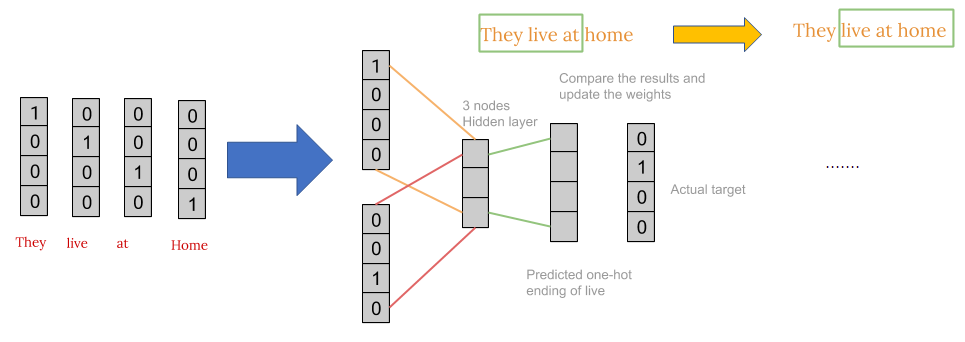
\includegraphics{./img/word-embedding-1.png}
\caption{image.png}
\end{figure}

    For example for a window size equal to three, we only consider three
words in a sentence. The middle word is to be predicted and the
surrounding two words are fed into the neural network as context. The
window is then slid and the process is repeated again. Finally, after
training the network repeatedly by sliding the window a shown above, we
get weights which we use to get the embeddings as shown below. Usually,
we take a window size of around 8-10 words and have a vector size of
300.

    

    \hypertarget{references-and-credits}{%
\section{References and Credits}\label{references-and-credits}}

\textbf{François Chollet}, ``Deep Learning with Python'', Manning
Publication, USA (2019)

\textbf{Brandon Rose},
\href{Document\%20Clustering\%20with\%20Python}{Document Clustering with
Python}


    % Add a bibliography block to the postdoc
    
    
    
\end{document}
